\documentclass[12pt, titlepage, french]{report}
%% -----------------------------
%% Encodage
%% -----------------------------
\usepackage[utf8]{inputenc}
\usepackage[T1]{fontenc}
\usepackage{babel}
\usepackage{lmodern}
%
%%% -----------------------------
%%% Définition de variables
%%% -----------------------------
%\def\auteur{Alec James van Rassel}
%\def\BackgroundColor{white}
%
%%% -----------------------------
%%% Margin and layout
%%% -----------------------------
%% Determine the margin for cheatsheet
%\usepackage[landscape, hmargin=1cm, vmargin=1.7cm]{geometry}
\usepackage{multicol}
\usepackage{sectsty}
\usepackage{titlesec}
%%% -----------------------------
%%%	Sections et chapitres
%%% -----------------------------
\titleformat{\chapter}
  {\normalfont\LARGE\bfseries}{\thechapter}{1em}{}
\titlespacing*{\chapter}{0pt}{3.5ex plus 1ex minus .2ex}{2.3ex plus .2ex}
\sectionfont{\color{cobalt}}
\subsectionfont{\color{indigo(web)}}
%%%
%%%	Avec cette commande, \section à le même comportement que \section* mais les sections apparaissent dans le TOC;
%%%	-	Ceci est appliqué aux sous-sections et sous-sous-sections, pas uniquement aux sections.
%
\setcounter{secnumdepth}{0}
%%%
%%%	Pour inclure les sous-sections dans la table des matières (TOC).
%%%
%%	Niveaux pour les classes book et report:
%%	-1:	part;			0:	chapter;		1:	section;			2:	subsection;	
%%	3:	subsubsection;	4:	paragraph;	5:	subparagraph;
%%	NOTE:	0 existe seulement pour les classes book et report et est part pour la class article.
%%%
\setcounter{tocdepth}{3}

%% -----------------------------
%% URL and links
%% -----------------------------
\usepackage{hyperref}
\usepackage{nameref}
\hypersetup{colorlinks = true, urlcolor = white, linkcolor = black}

%% -----------------------------
%% Document policy (en décommenter seulement une)
%% -----------------------------
%	\usepackage{concrete}
%	\usepackage{mathpazo}
%	\usepackage{frcursive} %% permet d'écrire en lettres attachées
%	\usepackage{aeguill}
%	\usepackage{mathptmx}
%	\usepackage{fourier} 

%% -----------------------------
%% Math configuration
%% -----------------------------
\usepackage[fleqn]{amsmath}
\usepackage{amsthm, amssymb, latexsym, amsfonts}
\usepackage{empheq}
\usepackage{numprint}
\usepackage{dsfont} % Pour avoir le symbole du domaine Z

%%% -----------------------------
%%% Raccourcis mathématiques
%%% -----------------------------
\newcommand{\reels}{\mathbb{R}}
\newcommand{\entiers}{\mathbb{Z}}
\newcommand{\naturels}{\mathbb{N}}
\newcommand{\eval}{\biggr \rvert}
\usepackage{cancel}
\newcommand{\derivee}[1]{\frac{\partial}{\partial #1}}
\newcommand{\prob}[1]{\Pr \left( #1 \right)}
\newcommand{\esp}[1]{\mathrm{E} \left[ #1 \right]} % espérance
\newcommand{\variance}[1]{\mathrm{Var} \left( #1   \right)}
\newcommand{\covar}[1]{\mathrm{Cov} \left( #1   \right)}
\newcommand{\laplace}{\mathcal{L}}
\newcommand{\deriv}[2][]{\frac{\partial^{#1}}{\partial #2^{#1}}}
\newcommand{\e}[1]{\mathrm{e}^{#1}}
\newcommand{\te}[1]{\text{exp}\left\{#1\right\}}
\DeclareMathSymbol{\shortminus}{\mathbin}{AMSa}{"39}

% To indicate equation number on a specific line in align environment
\newcommand\numberthis{\addtocounter{equation}{1}\tag{\theequation}}


%%% -----------------------------
%%% 	Paquetage de notation actuarielle
%%% -----------------------------
\usepackage{actuarialsymbol}
\usepackage{actuarialangle}

%%% -----------------------------
%%% Notation matricielle pour les symboles mathématiques
%%%
%%  (\bm{•})
%%% -----------------------------
\usepackage{bm}
%% Notation matricielle pour les variables
\newcommand{\matr}[1]{\mathbf{#1}}

%% -----------------------------
%% Configuration de tcolorbox
%% -----------------------------
\usepackage[most]{tcolorbox}
\tcbuselibrary{xparse}
\tcbuselibrary{breakable}
%%	-----------------------------
%%
%%	Arguments du paquetage
%%	+	breakable: allows box to be split over several pages
%%	+	segmentation style: To customize the \tcbline seperator
%%	
%%	-----------------------------
%%

%%
%% Coloured box "definition" for definitions
%%
\DeclareTColorBox{theorems}{ o}			% #1 parameter
{
	enhanced,
	title = #1,
	colback=bluebell, % color of the box
	colframe=blue(pigment),
	colbacktitle=blue!80!black,
	fonttitle = \bfseries,
	boxed title style={size=small,colframe=purple!50!black} ,
	attach boxed title to top center = {yshift=-3mm,yshifttext=-1mm},
	left=0pt,
  	right=0pt,
    box align=center,
    ams align*
%  	top=-10pt
}
\DeclareTColorBox{distributions}{ o }			% #1 parameter
{
	enhanced,
	title = #1,
	colback=ashgrey, % color of the box
%	colframe=blue(pigment),
	breakable,
	colframe=arsenic,	
	colbacktitle=aurometalsaurus,
	fonttitle = \bfseries,
	boxed title style={size=small,colframe=arsenic} ,
	attach boxed title to top center = {yshift=-3mm,yshifttext=-1mm},
%	left=0pt,
%  	right=0pt,
%    box align=center,
%    ams align*
%  	top=-10pt
}
\DeclareTColorBox{outcomes}{ o }			% #1 parameter
{
	enhanced,
	title = #1,
	colback=bluebell, % color of the box
%	colframe=blue(pigment),
%	colframe=asparagus,	
	breakable,
	colbacktitle=airforceblue,
	fonttitle = \bfseries,
	boxed title style={size=small,colframe=arsenic} ,
	attach boxed title to top center = {yshift=-3mm,yshifttext=-1mm},
%	left=0pt,
%  	right=0pt,
%    box align=center,
%    ams align*
%  	top=-10pt
}
\DeclareTColorBox{ASM_chapter}{ o }			% #1 parameter
{
	enhanced,
	title = #1,
	colback=darkseagreen, % color of the box
%	colframe=blue(pigment),
%	colframe=asparagus,	
	colbacktitle=britishracinggreen,
	fonttitle = \bfseries,
	boxed title style={size=small,colframe=arsenic} ,
	attach boxed title to top center = {yshift=-3mm,yshifttext=-1mm},
	segmentation style = {dashed, white},
	breakable
%	left=0pt,
%  	right=0pt,
%    box align=center,
%    ams align*
%  	top=-10pt
}
\DeclareTColorBox{YTB_vids}{ o }			% #1 parameter
{
	enhanced,
	title = #1,
	colback=red_rectangle, % color of the box
%	colframe=blue(pigment),
%	colframe=asparagus,	
	colbacktitle=lava,
	fonttitle = \bfseries,
	boxed title style={size=small,colframe=arsenic} ,
	attach boxed title to top center = {yshift=-3mm,yshifttext=-1mm},
	segmentation style = {dashed, white},
	breakable
%	left=0pt,
%  	right=0pt,
%    box align=center,
%    ams align*
%  	top=-10pt
}
%%
%% Coloured box "algo" for algorithms
%%
\newtcolorbox{algo}[ 1 ]
{
	colback = blue!5!white,
	colframe = blue!75!black,
	fonttitle = \bfseries,title=#1
}
%%
%% Coloured box "formula" for formulas
%%
\newtcolorbox{formula}[ 1 ]
{
	colback = green!5!white,
	colframe = darkseagreen,
	fonttitle = \bfseries,title=#1
}
%%
%% Coloured box "CHPT_SUMM" pour résumés des chapitres de l'ASM
%%
%\newtcolorbox[auto counter]{CHPT_SUMM}[ 2 ][] 	%pour ajouter du numérotage automatique
\newtcolorbox{CHPT_SUMM}[ 2 ][]
{
	colback = green!5!white,
	colframe = darkseagreen,
	breakable,
	enhanced,
	fonttitle = \bfseries,
%	title = Chapitre~\thetcbcounter: #2, 		pour inclure le numérotage automatique
	title = #2,
	#1
}
\newtcolorbox[list inside = CHPT]{CHPT_SUMM_AUTO}[ 2 ][]
{
	colback = green!5!white,
	colframe = darkseagreen,
	breakable,
	enhanced,
	fonttitle = \bfseries,
%	title = Chapitre~\thetcbcounter: #2, 		pour inclure le numérotage automatique
	title = #2,
	nameref = #2,
	after upper = {\addcontentsline{toc}{subsubsection}{#2}},
%	phantomlabel = {#2},
	#1
}
\newtcolorbox[auto counter, list inside = CHPT]{CHPT_SUMM_AUTO_NUMB}[ 2 ][]
{
	colback = green!5!white,
	colframe = darkseagreen,
	breakable,
	enhanced,
	fonttitle = \bfseries,
	title = Chapter~\thetcbcounter: #2, 		
%	title = #2,
	nameref = #2,
	after upper = {\addcontentsline{toc}{subsubsection}{\thetcbcounter: #2}},
%	phantomlabel = {#2},
	#1
}
%%
%% Coloured box "FORMULA_SUMM" pour résumés des formules de l'ASM
%%
\newtcolorbox{FORMULA_SUMM}[ 1 ]
{
	colback = babyblueeyes,
	colframe = airforceblue,
	breakable,
	fonttitle = \bfseries,title=#1
}
%%
%% Coloured box "YTB_SUMM" pour résumés des vidéos Youtube
%%
\newtcolorbox{YTB_SUMM}[ 2 ][]
{
	colback = red!5!white,
	colframe = darkterracotta,
	breakable,
	enhanced,
%	    frame hidden,
	fonttitle = \bfseries,
	title=#2,
	#1
}

%% -----------------------------
%% Graphiques et images
%% -----------------------------
\usepackage{graphicx}
\usepackage{pict2e}
\usepackage{tikz}

%%
%%	Crée un cercle
%%	Arguments:
%%	+	size
%%	+	colour
%%	
%%	Example:
%%	+	\tikzcircle[green, fill=blue]{1.5pt}
%%	+	\tikzcircle{2pt}
%%
\newcommand{\tikzcircle}[2][red,fill=red]{\tikz[baseline=-0.5ex]\draw[#1,radius=#2] (0,0) circle ;}

%%% -----------------------------
%%% insérer des pages pdf dans un document
%%% -----------------------------
\usepackage{pdfpages}

%%% -----------------------------
%%% Color configuration
%%% -----------------------------
\usepackage{color, soulutf8, colortbl}

%%% -----------------------------
%%%	Définitions de couleurs
%%% -----------------------------
\definecolor{darkterracotta}{rgb}{0.8, 0.31, 0.36}   % red pastel ish
\definecolor{lava}{rgb}{0.81, 0.06, 0.13}
\definecolor{wildwatermelon}{rgb}{0.99, 0.42, 0.52}  % red ish
\definecolor{bostonuniversityred}{rgb}{0.8, 0.0, 0.0} % rich red
\definecolor{asparagus}{rgb}{0.53, 0.66, 0.42}		% sorta militarygreen but pastel
\definecolor{darkseagreen}{rgb}{0.56, 0.74, 0.56}    % pastel light green
\definecolor{britishracinggreen}{rgb}{0.0, 0.26, 0.15} %dark green
\definecolor{airforceblue}{rgb}{0.36, 0.54, 0.66}	% nice teal blue pastel
\definecolor{babyblueeyes}{rgb}{0.63, 0.79, 0.95}	% pastel blue-ish
\definecolor{applegreen}{rgb}{0.55, 0.71, 0.0}		% green with some aqua
\definecolor{indigo(web)}{rgb}{0.29, 0.0, 0.51}
\definecolor{cobalt}{rgb}{0.0, 0.28, 0.67}
\definecolor{azure(colorwheel)}{rgb}{0.0, 0.5, 1.0}
\definecolor{darkpastelpurple}{rgb}{0.59, 0.44, 0.84}
\definecolor{darkgreen}{rgb}{0.0, 0.2, 0.13}			
\definecolor{burntorange}{rgb}{0.8, 0.33, 0.0}		
\definecolor{burntsienna}{rgb}{0.91, 0.45, 0.32}		
\definecolor{ao(english)}{rgb}{0.0, 0.5, 0.0}		% ACT-2003
\definecolor{amber(sae/ece)}{rgb}{1.0, 0.49, 0.0} 	% ACT-2004
\definecolor{green_rectangle}{RGB}{131, 176, 84}		% ACT-2004
\definecolor{red_rectangle}{RGB}{241,112,113}		% ACT-2004
\definecolor{blue_rectangle}{RGB}{83, 84, 244}		% ACT-2004
\definecolor{blue(pigment)}{rgb}{0.2, 0.2, 0.6}
\definecolor{bluebell}{rgb}{0.64, 0.64, 0.82}
\definecolor{amethyst}{rgb}{0.6, 0.4, 0.8}
\definecolor{amethyst-light}{rgb}{0.6, 0.4, 0.8}
\definecolor{aurometalsaurus}{rgb}{0.43, 0.5, 0.5}
\definecolor{arsenic}{rgb}{0.23, 0.27, 0.29}			%	dark black-grey ish pastel
\definecolor{ashgrey}{rgb}{0.7, 0.75, 0.71}
%
% Useful shortcuts for coloured text
%
\newcommand{\orange}{\textcolor{orange}}
\newcommand{\red}{\textcolor{red}}
\newcommand{\cyan}{\textcolor{cyan}}
\newcommand{\blue}{\textcolor{blue}}
\newcommand{\green}{\textcolor{green}}
\newcommand{\purple}{\textcolor{magenta}}
\newcommand{\yellow}{\textcolor{yellow}}

%% -----------------------------
%% Enumerate environment configuration
%% -----------------------------
%
% Custum enumerate & itemize Package
%
\usepackage{enumitem}
%
% French Setup for itemize function
%
\frenchbsetup{StandardItemLabels=true}
%
% Change default label for itemize
%
\renewcommand{\labelitemi}{\faAngleRight}


%% -----------------------------
%% Tabular column type configuration
%% -----------------------------
\newcolumntype{C}{>{$}c<{$}} % math-mode version of "l" column type
\newcolumntype{L}{>{$}l<{$}} % math-mode version of "l" column type
\newcolumntype{R}{>{$}r<{$}} % math-mode version of "l" column type
\newcolumntype{f}{>{\columncolor{green!20!white}}p{1cm}}
\newcolumntype{g}{>{\columncolor{green!40!white}}m{1.2cm}}
\newcolumntype{a}{>{\columncolor{red!20!white}$}p{2cm}<{$}}	% ACT-2005
% configuration to force a line break within a single cell
\usepackage{makecell}


%% -----------------------------
%% Fontawesome for special symbols
%% -----------------------------
\usepackage{fontawesome}

%
%%% -----------------------------
%%% Footer/Header Customization
%%% -----------------------------
%\usepackage{lastpage}
%\usepackage{fancyhdr}
%\pagestyle{fancy}
%%
%% Page background color
%%
%\pagecolor{\BackgroundColor}


%% END OF PREAMBLE
% ---------------------------------------------
% ---------------------------------------------
%% -----------------------------
%% Section Font customization
%% -----------------------------
\title{
	Guide d'étude	\\
	\large Examen SRM: Statistics for Risk Modeling 	\\
	Society of Actuaries (SOA)}
\vspace{-8ex}
\date{}
\author{Alec James van Rassel}

\begin{document}

\maketitle

\tableofcontents

\clearpage

\part*{Préliminaires}

\begin{YTB_vids}[Vidéos YouTube]
\begin{itemize}
	\item	\href{https://www.youtube.com/watch?v=bsZGt-caXO4}{StatQuest: One or Two Tailed P-Values}
	\item	\href{https://www.youtube.com/watch?v=KS6KEWaoOOE}{Khan Academy: P-values and significance tests}
\end{itemize}
\end{YTB_vids}

\begin{YTB_SUMM}{\href{https://www.youtube.com/watch?v=bsZGt-caXO4}{StatQuest: One or Two Tailed P-Values}}
\begin{itemize}
	\item	\textbf{Test} new treatment \tikzcircle[burntorange, fill=burntorange]{3pt} vs old treatment \tikzcircle[black, fill=black]{3pt}
	\begin{itemize}
		\item	One-tailed: $\mathcal{H}_{0}:$ The new treatment \tikzcircle[burntorange, fill=burntorange]{3pt} is \textit{better} than the old treatment \tikzcircle[black, fill=black]{3pt}.
		\item	Two-tailed: $\mathcal{H}_{0}:$ The new treatment \tikzcircle[burntorange, fill=burntorange]{3pt} is \textit{better}, \textit{worse} or \textit{not significantly different} than the old treatment \tikzcircle[black, fill=black]{3pt}.
	\end{itemize}
	\item	\textbf{P-Hacking}
	\begin{itemize}
		\item	Deciding to test if the new treatment \tikzcircle[burntorange, fill=burntorange]{3pt} is \textit{better} rather than \textit{better}, \textit{worse} or \textit{not significantly different} than the old treatment \tikzcircle[black, fill=black]{3pt} \textit{after} seeing the skewed distribution.
	\end{itemize}
	\item	\textbf{False Positive} \textit{(recall the image of the normal distribution with the points)}
	\begin{itemize}
		\item	Usually, the two samples for \tikzcircle[burntorange, fill=burntorange]{3pt} and \tikzcircle[black, fill=black]{3pt} overlap (recall image where they're overlapping) but it can happen that they don't (recall image where they're spaced out) in which case the p-value is less than $0.05$ and we have a \textbf{\textit{false positive}}.
	\end{itemize}
	\item	To decide which $t$ test to use, ask ourselves \textbf{what we want to learn from the test} and then decide.
\end{itemize}
\end{YTB_SUMM}

\begin{YTB_SUMM}{\href{https://www.youtube.com/watch?v=KS6KEWaoOOE}{Khan Academy: P-values and significance tests}}
\begin{itemize}
	\item	Test de signification
	\begin{enumerate}[label=\roman*]
		\item	Déterminer la question
		\item	Établir les connus
	\end{enumerate}
	\begin{enumerate}
		\item	Définir les hypothèses $\mathcal{H}_{0}$ et $\mathcal{H}_{a}$
		\item	Établir un niveau de signification $\alpha$ (souvent $0.05$)
		\item	Obtenir un échantillon
		\item	Trouver la p-value
		\begin{itemize}
			\item	p-value = Pr\{ statistique de test si $\mathcal{H}_{0}$ est vrai \} $\neq$  Pr\{ $\mathcal{H}_{0}$ est vrai sachant la statistique de test \}
		\end{itemize}
		\item	Décider
		\begin{itemize}
			\item	Si p-value $< \alpha$  alors on rejète l'hypothèse nulle
			\item	Si p-value $\geq \alpha$ alors on ne peut pas rejeter l'hypothèse nulle
		\end{itemize}
	\end{enumerate}
\end{itemize}
\end{YTB_SUMM}

\clearpage

\part*{Sujets à l'étude}

\chapter[Basics of statistical learning]{Basics of statistical learning (7.5\% à 12.5\%)}

%\addcontentsline{toc}{subsection}{Information}
\subsubsection{Information}

\begin{distributions}[Objective]
Understand key concepts of statistical learning
\end{distributions}

\begin{outcomes}[Learning outcomes]
\begin{enumerate}
	\item	Expliquer les différents types de problèmes, et différentes méthodes, de modélisation. Y compris: 
	\begin{itemize}
		\item	Apprentissage supervisé vs non-supervisé
		\item	Régression vs classification	
	\end{itemize}
	\item	Expliquer les méthodes courantes pour évaluer la précision d'un modèle.
	\item	Utiliser les méthodes de base d'analyse exploratoire de données y compris la validation et vérification de données.
\end{enumerate}
\end{outcomes}

\begin{ASM_chapter}[Related lessons ASM]
\begin{enumerate}
	\item	Basics of Statistical Learning
\end{enumerate}
\end{ASM_chapter}

\begin{YTB_vids}[Vidéos YouTube]
\begin{itemize}
	\item	\href{https://www.youtube.com/watch?v=Gv9_4yMHFhI&list=PLblh5JKOoLUICTaGLRoHQDuF_7q2GfuJF&index=2&t=0s}{StatQuest: A Gentle Introduction to Machine Learning}
	\item	\href{https://www.youtube.com/watch?v=EuBBz3bI-aA&list=PLblh5JKOoLUICTaGLRoHQDuF_7q2GfuJF&index=6}{StatQuest: Machine Learning Fundamentals: Bias and Variance}
	\item	\href{https://www.youtube.com/watch?v=IFKQLDmRK0Y&feature=youtu.be}{StatQuest: StatQuest: Quantiles and Percentiles, Clearly Explained!!!}
	\item	\href{https://www.youtube.com/watch?v=okjYjClSjOg&list=PLblh5JKOoLUIcdlgu78MnlATeyx4cEVeR&index=20}{StatQuest: Quantile-Quantile plots (QQ plots), clearly explained}
	\item	\href{https://www.youtube.com/watch?v=ecjN6Xpv6SE&feature=youtu.be}{StatQuest: Quantile Normalization}
\end{itemize}
\end{YTB_vids}

\begin{CHPT_SUMM}{1. Basics of Statistical Learning}
	\begin{itemize}
		\item	Définitions de base
		\item	Comparaisons
		\begin{itemize}
			\item	Prévision vs inférence
			\item	Paramétrique vs non-paramétrique 
			\item	Flexibilité vs interprétabilité
			\item	Apprentissage supervisé vs non-supervisé
			\item	Régression vs classification
			\item	Biais vs variance 
		\end{itemize}
		\item	Types de variables
		\begin{itemize}
			\item	Continue
			\item	Catégorique
			\begin{itemize}
				\item[]	S'il y a une ordre logique, c'est \textit{ordinal} sinon nominal.
			\end{itemize}
			\item	Comptage
		\end{itemize}
		\item	Graphiques (scatter, box, qq)
	\end{itemize}
\end{CHPT_SUMM}


\begin{YTB_SUMM}{\href{https://www.youtube.com/watch?v=Gv9_4yMHFhI&list=PLblh5JKOoLUICTaGLRoHQDuF_7q2GfuJF&index=2&t=0s}{StatQuest: A Gentle Introduction to Machine Learning}}
\begin{itemize}
	\item	Le but de l'apprentissage machine est de faire des \textbf{prévisions}. 
	\item	Les \textit{arbres de décisions} peuvent être utilisés pour la prévision ou la \textbf{classification} et la régression pour la prévision.
	\item	Peut importe la méthode, l'important est de mesurer la \textit{\textbf{précision} des prévisions}.
	\item	On peut donc tester notre méthode avec du \textbf{testing data}.
	\item	\textbf{Bias-Variance tradeoff}: Être bien ajusté, mais avoir des mauvaise prévisions.
\end{itemize}
\end{YTB_SUMM}

\begin{YTB_SUMM}{\href{https://www.youtube.com/watch?v=EuBBz3bI-aA&list=PLblh5JKOoLUICTaGLRoHQDuF_7q2GfuJF&index=6}{StatQuest: Machine Learning Fundamentals: Bias and Variance}}
\begin{itemize}
	\item	\textbf{Biais}: Inhabilité pour une méthode de prévision de capturer la vraie relation. Par exemple:
	\begin{itemize}
		\item	Essayer de fit une droite aux points du vidéo; évidemment elle ne peut pas reproduire la vraie relation \textbf{VS} une squiggly line qui peut avec little to no biais.
		\item	Alors, la squiggly line sera mieux ajusté aux données d'entrainement mais pas aux testing data; alias, elle sera \textbf{overfitted}.
	\end{itemize}
	\item	\textbf{Variance}: Variance de l'ajustement entre ensembles de données.
	\begin{itemize}
		\item	La squiggly line aura une variance très élevée mais pas la droite; la droite est cohérente et aura toujours un \textbf{SSE} similaire.
	\end{itemize}
	\item	On cherche donc la meilleur combinaison des deux méthodes. Plusieurs méthodes existent pour la trouver dont la \textbf{régularisation}, le \textit{boosting} et le \textit{bagging}.
\end{itemize}
\end{YTB_SUMM}

\begin{YTB_SUMM}{\href{https://www.youtube.com/watch?v=IFKQLDmRK0Y&feature=youtu.be}{StatQuest: StatQuest: Quantiles and Percentiles, Clearly Explained!!!}}
Visualise the chart with the 15 points to which we add the lines.
\begin{enumerate}
	\item	The \textbf{median} is a quantile because it splits the data into 2 equally sized groups.
	\begin{itemize}
		\item	The (0.5 | 50\%) quantile value is 4.5.
	\end{itemize}
	\item	The (0.25 | 25\%) quantile is such that (25\% | a quarter) of the points are less than it.
	\item	\textbf{Technically}, quantiles are line which divide the data into equally sized groups.
	\item	\textbf{Technically}, percentiles are just quantiles which divide the data into 100 equally sized groups.
	\begin{itemize}
		\item	In practice, terminology is much more flexible;
		\item	Even if there's less than 100\%, we still call the ( median | 50\% quantile) the 50$^{th}$ percentile.
		\item	To calculate a quantile / percentile, just calculate how many values are less than it.
	\end{itemize}
	\item	There are many other ways to calculate quantiles, R has 9 just by itself!
	\item	The lesson however, is that the smaller the sample the more variable the results.
\end{enumerate}
\end{YTB_SUMM}

\begin{YTB_SUMM}{\href{https://www.youtube.com/watch?v=okjYjClSjOg&list=PLblh5JKOoLUIcdlgu78MnlATeyx4cEVeR&index=20}{StatQuest: Quantile-Quantile plots (QQ plots), clearly explained}}
\begin{enumerate}
	\item	Give each data point it's quantile.
	\item	Get a normal curve.
	\item	Add all the quantiles obtained to the curve.
	\begin{itemize}
		\item	That's to say the percentage and not the value.
	\end{itemize}
	\item	Plot QQ graph.
	\begin{itemize}
		\item	If the data were normal, most data points would be on the line;
		\item	If the fit is not good, can try a different distribution;
		\item	Thus, can use the QQ plot to see which distribution fits the data.
	\end{itemize}
\end{enumerate}
\begin{itemize}
	\item	Could also use the QQ plot to compare 2 datasets.
	\item	For example, if the second one had less data points we could use quartiles instead!
	\item	We add the points at the intersection of the 2 datasets' quantiles and add a straight line.
\end{itemize}
\end{YTB_SUMM}

\begin{YTB_SUMM}{\href{https://www.youtube.com/watch?v=ecjN6Xpv6SE&feature=youtu.be}{StatQuest: Quantile Normalization}}

\tikzset{every picture/.style={line width=0.75pt}} %set default line width to 0.75pt        
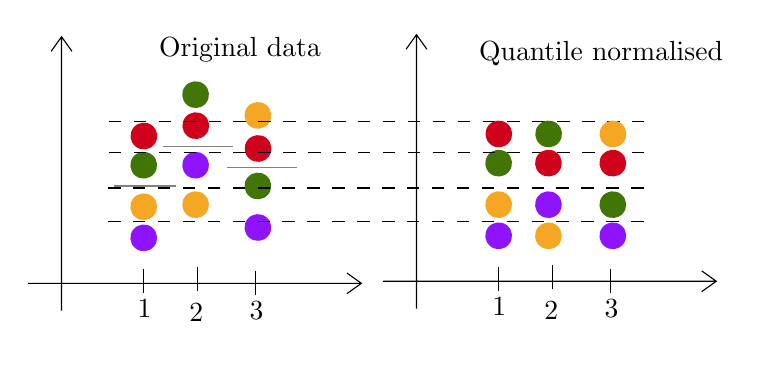
\begin{tikzpicture}[x=0.75pt,y=0.75pt,yscale=-1,xscale=1]
%uncomment if require: \path (0,195.33333206176758); %set diagram left start at 0, and has height of 195.33333206176758

%Shape: Axis 2D [id:dp4071697184363743] 
\draw  (31,131.8) -- (191.5,131.8)(47.05,13) -- (47.05,145) (184.5,126.8) -- (191.5,131.8) -- (184.5,136.8) (42.05,20) -- (47.05,13) -- (52.05,20)  ;
%Flowchart: Connector [id:dp47796321909784445] 
\draw  [draw opacity=0][fill={rgb, 255:red, 65; green, 117; blue, 5 }  ,fill opacity=1 ] (90.71,69.91) .. controls (87.96,67.66) and (83.9,68.07) .. (81.65,70.83) .. controls (79.4,73.59) and (79.81,77.64) .. (82.57,79.89) .. controls (85.33,82.14) and (89.39,81.73) .. (91.63,78.97) .. controls (93.88,76.21) and (93.47,72.16) .. (90.71,69.91) -- cycle ;
%Flowchart: Connector [id:dp775136720322851] 
\draw  [draw opacity=0][fill={rgb, 255:red, 144; green, 19; blue, 254 }  ,fill opacity=1 ] (90.71,104.91) .. controls (87.96,102.66) and (83.9,103.07) .. (81.65,105.83) .. controls (79.4,108.59) and (79.81,112.64) .. (82.57,114.89) .. controls (85.33,117.14) and (89.39,116.73) .. (91.63,113.97) .. controls (93.88,111.21) and (93.47,107.16) .. (90.71,104.91) -- cycle ;
%Flowchart: Connector [id:dp479825470074684] 
\draw  [draw opacity=0][fill={rgb, 255:red, 245; green, 166; blue, 35 }  ,fill opacity=1 ] (90.71,89.91) .. controls (87.96,87.66) and (83.9,88.07) .. (81.65,90.83) .. controls (79.4,93.59) and (79.81,97.64) .. (82.57,99.89) .. controls (85.33,102.14) and (89.39,101.73) .. (91.63,98.97) .. controls (93.88,96.21) and (93.47,92.16) .. (90.71,89.91) -- cycle ;
%Flowchart: Connector [id:dp8772408378730552] 
\draw  [draw opacity=0][fill={rgb, 255:red, 208; green, 2; blue, 27 }  ,fill opacity=1 ] (90.79,55.84) .. controls (88.03,53.6) and (83.98,54.01) .. (81.73,56.77) .. controls (79.48,59.52) and (79.89,63.58) .. (82.65,65.83) .. controls (85.41,68.08) and (89.46,67.66) .. (91.71,64.91) .. controls (93.96,62.15) and (93.55,58.09) .. (90.79,55.84) -- cycle ;
%Flowchart: Connector [id:dp7273952498995546] 
\draw  [draw opacity=0][fill={rgb, 255:red, 65; green, 117; blue, 5 }  ,fill opacity=1 ] (115.71,35.91) .. controls (112.96,33.66) and (108.9,34.07) .. (106.65,36.83) .. controls (104.4,39.59) and (104.81,43.64) .. (107.57,45.89) .. controls (110.33,48.14) and (114.39,47.73) .. (116.63,44.97) .. controls (118.88,42.21) and (118.47,38.16) .. (115.71,35.91) -- cycle ;
%Flowchart: Connector [id:dp21583380928952534] 
\draw  [draw opacity=0][fill={rgb, 255:red, 144; green, 19; blue, 254 }  ,fill opacity=1 ] (115.71,69.91) .. controls (112.96,67.66) and (108.9,68.07) .. (106.65,70.83) .. controls (104.4,73.59) and (104.81,77.64) .. (107.57,79.89) .. controls (110.33,82.14) and (114.39,81.73) .. (116.63,78.97) .. controls (118.88,76.21) and (118.47,72.16) .. (115.71,69.91) -- cycle ;
%Flowchart: Connector [id:dp367353299394227] 
\draw  [draw opacity=0][fill={rgb, 255:red, 245; green, 166; blue, 35 }  ,fill opacity=1 ] (115.71,88.91) .. controls (112.96,86.66) and (108.9,87.07) .. (106.65,89.83) .. controls (104.4,92.59) and (104.81,96.64) .. (107.57,98.89) .. controls (110.33,101.14) and (114.39,100.73) .. (116.63,97.97) .. controls (118.88,95.21) and (118.47,91.16) .. (115.71,88.91) -- cycle ;
%Flowchart: Connector [id:dp9918881154852264] 
\draw  [draw opacity=0][fill={rgb, 255:red, 208; green, 2; blue, 27 }  ,fill opacity=1 ] (115.79,50.84) .. controls (113.03,48.6) and (108.98,49.01) .. (106.73,51.77) .. controls (104.48,54.52) and (104.89,58.58) .. (107.65,60.83) .. controls (110.41,63.08) and (114.46,62.66) .. (116.71,59.91) .. controls (118.96,57.15) and (118.55,53.09) .. (115.79,50.84) -- cycle ;
%Flowchart: Connector [id:dp8737482771717215] 
\draw  [draw opacity=0][fill={rgb, 255:red, 65; green, 117; blue, 5 }  ,fill opacity=1 ] (145.71,79.91) .. controls (142.96,77.66) and (138.9,78.07) .. (136.65,80.83) .. controls (134.4,83.59) and (134.81,87.64) .. (137.57,89.89) .. controls (140.33,92.14) and (144.39,91.73) .. (146.63,88.97) .. controls (148.88,86.21) and (148.47,82.16) .. (145.71,79.91) -- cycle ;
%Flowchart: Connector [id:dp8886502638185938] 
\draw  [draw opacity=0][fill={rgb, 255:red, 144; green, 19; blue, 254 }  ,fill opacity=1 ] (145.71,99.91) .. controls (142.96,97.66) and (138.9,98.07) .. (136.65,100.83) .. controls (134.4,103.59) and (134.81,107.64) .. (137.57,109.89) .. controls (140.33,112.14) and (144.39,111.73) .. (146.63,108.97) .. controls (148.88,106.21) and (148.47,102.16) .. (145.71,99.91) -- cycle ;
%Flowchart: Connector [id:dp12839712018807292] 
\draw  [draw opacity=0][fill={rgb, 255:red, 245; green, 166; blue, 35 }  ,fill opacity=1 ] (145.71,45.91) .. controls (142.96,43.66) and (138.9,44.07) .. (136.65,46.83) .. controls (134.4,49.59) and (134.81,53.64) .. (137.57,55.89) .. controls (140.33,58.14) and (144.39,57.73) .. (146.63,54.97) .. controls (148.88,52.21) and (148.47,48.16) .. (145.71,45.91) -- cycle ;
%Flowchart: Connector [id:dp22911262187569625] 
\draw  [draw opacity=0][fill={rgb, 255:red, 208; green, 2; blue, 27 }  ,fill opacity=1 ] (145.79,61.84) .. controls (143.03,59.6) and (138.98,60.01) .. (136.73,62.77) .. controls (134.48,65.52) and (134.89,69.58) .. (137.65,71.83) .. controls (140.41,74.08) and (144.46,73.66) .. (146.71,70.91) .. controls (148.96,68.15) and (148.55,64.09) .. (145.79,61.84) -- cycle ;
%Straight Lines [id:da7437423031647632] 
\draw    (140.63,126) -- (140.63,137.3) ;


%Straight Lines [id:da3500611217714251] 
\draw    (112.63,124) -- (112.63,135.3) ;


%Straight Lines [id:da4946427268334965] 
\draw    (86.63,125) -- (86.63,136.3) ;


%Straight Lines [id:da39022019683066134] 
\draw [color={rgb, 255:red, 128; green, 128; blue, 128 }  ,draw opacity=1 ]   (126.96,75.91) -- (160.46,75.91) ;


%Straight Lines [id:da3674903648864307] 
\draw [color={rgb, 255:red, 128; green, 128; blue, 128 }  ,draw opacity=1 ]   (95.96,65.91) -- (129.46,65.91) ;


%Straight Lines [id:da08905855224756842] 
\draw [color={rgb, 255:red, 128; green, 128; blue, 128 }  ,draw opacity=1 ]   (72.5,84.89) -- (102.32,84.89) ;


%Straight Lines [id:da8838665914886257] 
\draw  [dash pattern={on 4.5pt off 4.5pt}]  (69.89,53.9) -- (330.83,53.9) ;


%Shape: Axis 2D [id:dp5094712129345804] 
\draw  (202,130.8) -- (362.5,130.8)(218.05,12) -- (218.05,144) (355.5,125.8) -- (362.5,130.8) -- (355.5,135.8) (213.05,19) -- (218.05,12) -- (223.05,19)  ;
%Flowchart: Connector [id:dp9701135659715163] 
\draw  [draw opacity=0][fill={rgb, 255:red, 65; green, 117; blue, 5 }  ,fill opacity=1 ] (261.71,68.91) .. controls (258.96,66.66) and (254.9,67.07) .. (252.65,69.83) .. controls (250.4,72.59) and (250.81,76.64) .. (253.57,78.89) .. controls (256.33,81.14) and (260.39,80.73) .. (262.63,77.97) .. controls (264.88,75.21) and (264.47,71.16) .. (261.71,68.91) -- cycle ;
%Flowchart: Connector [id:dp19815624460829806] 
\draw  [draw opacity=0][fill={rgb, 255:red, 144; green, 19; blue, 254 }  ,fill opacity=1 ] (261.71,103.91) .. controls (258.96,101.66) and (254.9,102.07) .. (252.65,104.83) .. controls (250.4,107.59) and (250.81,111.64) .. (253.57,113.89) .. controls (256.33,116.14) and (260.39,115.73) .. (262.63,112.97) .. controls (264.88,110.21) and (264.47,106.16) .. (261.71,103.91) -- cycle ;
%Flowchart: Connector [id:dp5444970436061509] 
\draw  [draw opacity=0][fill={rgb, 255:red, 245; green, 166; blue, 35 }  ,fill opacity=1 ] (261.71,88.91) .. controls (258.96,86.66) and (254.9,87.07) .. (252.65,89.83) .. controls (250.4,92.59) and (250.81,96.64) .. (253.57,98.89) .. controls (256.33,101.14) and (260.39,100.73) .. (262.63,97.97) .. controls (264.88,95.21) and (264.47,91.16) .. (261.71,88.91) -- cycle ;
%Flowchart: Connector [id:dp4129473941443531] 
\draw  [draw opacity=0][fill={rgb, 255:red, 208; green, 2; blue, 27 }  ,fill opacity=1 ] (261.79,54.84) .. controls (259.03,52.6) and (254.98,53.01) .. (252.73,55.77) .. controls (250.48,58.52) and (250.89,62.58) .. (253.65,64.83) .. controls (256.41,67.08) and (260.46,66.66) .. (262.71,63.91) .. controls (264.96,61.15) and (264.55,57.09) .. (261.79,54.84) -- cycle ;
%Straight Lines [id:da49630299738040096] 
\draw    (311.63,125) -- (311.63,136.3) ;


%Straight Lines [id:da3409139232705698] 
\draw    (283.63,123) -- (283.63,134.3) ;


%Straight Lines [id:da9094998541395087] 
\draw    (257.63,124) -- (257.63,135.3) ;


%Straight Lines [id:da2261043426810294] 
\draw  [dash pattern={on 4.5pt off 4.5pt}]  (69.89,68.9) -- (330.83,68.9) ;


%Straight Lines [id:da5824626395640147] 
\draw  [dash pattern={on 4.5pt off 4.5pt}]  (69.5,85.89) -- (330.44,85.89) ;


%Straight Lines [id:da7047611196217718] 
\draw  [dash pattern={on 4.5pt off 4.5pt}]  (69.5,101.89) -- (330.44,101.89) ;


%Flowchart: Connector [id:dp8893219442781508] 
\draw  [draw opacity=0][fill={rgb, 255:red, 208; green, 2; blue, 27 }  ,fill opacity=1 ] (285.71,68.91) .. controls (282.96,66.66) and (278.9,67.07) .. (276.65,69.83) .. controls (274.4,72.59) and (274.81,76.64) .. (277.57,78.89) .. controls (280.33,81.14) and (284.39,80.73) .. (286.63,77.97) .. controls (288.88,75.21) and (288.47,71.16) .. (285.71,68.91) -- cycle ;
%Flowchart: Connector [id:dp3959621528301924] 
\draw  [draw opacity=0][fill={rgb, 255:red, 245; green, 166; blue, 35 }  ,fill opacity=1 ] (285.71,103.91) .. controls (282.96,101.66) and (278.9,102.07) .. (276.65,104.83) .. controls (274.4,107.59) and (274.81,111.64) .. (277.57,113.89) .. controls (280.33,116.14) and (284.39,115.73) .. (286.63,112.97) .. controls (288.88,110.21) and (288.47,106.16) .. (285.71,103.91) -- cycle ;
%Flowchart: Connector [id:dp1772629821607905] 
\draw  [draw opacity=0][fill={rgb, 255:red, 144; green, 19; blue, 254 }  ,fill opacity=1 ] (285.71,88.91) .. controls (282.96,86.66) and (278.9,87.07) .. (276.65,89.83) .. controls (274.4,92.59) and (274.81,96.64) .. (277.57,98.89) .. controls (280.33,101.14) and (284.39,100.73) .. (286.63,97.97) .. controls (288.88,95.21) and (288.47,91.16) .. (285.71,88.91) -- cycle ;
%Flowchart: Connector [id:dp852667519103441] 
\draw  [draw opacity=0][fill={rgb, 255:red, 65; green, 117; blue, 5 }  ,fill opacity=1 ] (285.79,54.84) .. controls (283.03,52.6) and (278.98,53.01) .. (276.73,55.77) .. controls (274.48,58.52) and (274.89,62.58) .. (277.65,64.83) .. controls (280.41,67.08) and (284.46,66.66) .. (286.71,63.91) .. controls (288.96,61.15) and (288.55,57.09) .. (285.79,54.84) -- cycle ;
%Flowchart: Connector [id:dp42164729435747383] 
\draw  [draw opacity=0][fill={rgb, 255:red, 208; green, 2; blue, 27 }  ,fill opacity=1 ] (316.71,68.91) .. controls (313.96,66.66) and (309.9,67.07) .. (307.65,69.83) .. controls (305.4,72.59) and (305.81,76.64) .. (308.57,78.89) .. controls (311.33,81.14) and (315.39,80.73) .. (317.63,77.97) .. controls (319.88,75.21) and (319.47,71.16) .. (316.71,68.91) -- cycle ;
%Flowchart: Connector [id:dp1353268144862132] 
\draw  [draw opacity=0][fill={rgb, 255:red, 144; green, 19; blue, 254 }  ,fill opacity=1 ] (316.71,103.91) .. controls (313.96,101.66) and (309.9,102.07) .. (307.65,104.83) .. controls (305.4,107.59) and (305.81,111.64) .. (308.57,113.89) .. controls (311.33,116.14) and (315.39,115.73) .. (317.63,112.97) .. controls (319.88,110.21) and (319.47,106.16) .. (316.71,103.91) -- cycle ;
%Flowchart: Connector [id:dp5695947224831286] 
\draw  [draw opacity=0][fill={rgb, 255:red, 65; green, 117; blue, 5 }  ,fill opacity=1 ] (316.71,88.91) .. controls (313.96,86.66) and (309.9,87.07) .. (307.65,89.83) .. controls (305.4,92.59) and (305.81,96.64) .. (308.57,98.89) .. controls (311.33,101.14) and (315.39,100.73) .. (317.63,97.97) .. controls (319.88,95.21) and (319.47,91.16) .. (316.71,88.91) -- cycle ;
%Flowchart: Connector [id:dp5282331948658441] 
\draw  [draw opacity=0][fill={rgb, 255:red, 245; green, 166; blue, 35 }  ,fill opacity=1 ] (316.79,54.84) .. controls (314.03,52.6) and (309.98,53.01) .. (307.73,55.77) .. controls (305.48,58.52) and (305.89,62.58) .. (308.65,64.83) .. controls (311.41,67.08) and (315.46,66.66) .. (317.71,63.91) .. controls (319.96,61.15) and (319.55,57.09) .. (316.79,54.84) -- cycle ;

% Text Node
\draw (87,144) node   [align=left] {1};
% Text Node
\draw (112,154) node   [align=left] {2\\};
% Text Node
\draw (141,145) node   [align=left] {3};
% Text Node
\draw (258,143) node   [align=left] {1};
% Text Node
\draw (283,153) node   [align=left] {2\\};
% Text Node
\draw (312,144) node   [align=left] {3};
% Text Node
\draw (307,21) node   [align=left] {Quantile normalised};
% Text Node
\draw (133,19) node   [align=left] {Original data};


\end{tikzpicture}

The idea for quantile normalisation ressembles the offset in linear regression. You account for differences in samples to adequately compare them.
\begin{enumerate}
	\item[]	 To compensate for the differences in lightbulb intensity across samples, want to normalise the data points; you can see the difference in means across all three \textcolor{gray}{in gray}.
	\item	Focus on the maximum value of each sample and take the mean.
	\item[]	Extend this mean onto the new plot and that becomes the new value for all 3 samples.
	\item	Repeat for all the points.
	\item[]	The end result is that the \textbf{values are all the same} but the \textbf{order of the colours is maintained} enabling an adequate comparison.
\end{enumerate}
\end{YTB_SUMM}

\newpage
\chapter[Linear Models]{Linear Models (40\% à 50\%)}

\subsubsection{Information}

\begin{distributions}[Objective]
Understand key concepts concerning Generalized Linear Models
\end{distributions}

\begin{outcomes}[Learning outcomes]
\begin{enumerate}
	\item	Décrire et expliquer les composantes de la famille exponentielle et des fonctions de lien.
	\item	Estimer les paramètres par Least Squares et maximum de vraisemblance.
	\item	Interpréter les tests de vérification pour l'ajustement de modèle et la vérification des postulats graphiquement et numériquement.
	\item	Sélectionner un modèle approprié en prenant en compte:
	\begin{itemize}
		\item	Distributions et fonctions de lien
		\item	Transformations de variables, et leurs interactions
		\item	Statistique (du khi-carré) de Pearson
		\item	Tests $t$ et $F$
		\item	AIC et BIC
		\item	Test du Rapport de Vraisemblance (TRV)
	\end{itemize}
	\item	Interpréter les résultats du modèle dans le cadre de son utilisation pour résoudre aux problèmes d'affaires sous-jacents
	\item	Calculer et interpréter les valeurs prédites ainsi que les intervalles de confiance et de prévision.
	\item	Comprendre que d'autres méthodes peuvent différer du modèle OLS comme la régression Lasso, Ridge et KNN.
\end{enumerate}
\end{outcomes}

\begin{ASM_chapter}[Related lessons ASM]
\begin{enumerate}
  \setcounter{enumi}{1}
	\item	Linear Regression:  Estimating parameters
	\item	Linear Regression:  Standard Error, $R^{2}$, and $t$ statistic
	\item	Linear Regression:  $F$ statistic
	\tcbline
	\item	Linear Regression:  Validation
	\item	Resampling methods
	\item	Linear Regression:  Subset Selection
	\item	Linear Regression:  Shrinkage and Dimension Reduction
	\tcbline
	\item	Linear Regression:  Predictions
	\item	Interpreting Regression Results
	\tcbline
	\item	Generalized Linear Models:  Basics
	\item	Generalized Linear Models:  Categorical Response
	\item	Generalized Linear Models:  Count Response
	\item	Generalized Linear Models:  Measures of Fit
\end{enumerate}
\end{ASM_chapter}

\begin{YTB_vids}[Vidéos YouTube]
\begin{itemize}
	\item	\href{https://www.youtube.com/watch?v=2QeDRsxSF9M&t=369s}{Khan Academy: Pearson's chi square test (goodness of fit)}
	\item	\href{https://www.youtube.com/watch?v=PaFPbb66DxQ&list=PLblh5JKOoLUIzaEkCLIUxQFjPIlapw8nU&index=1}{StatQuest: Fitting a line to data, aka least squares, aka linear regression}
	\item	\href{https://www.youtube.com/watch?v=2AQKmw14mHM&list=PLblh5JKOoLUIzaEkCLIUxQFjPIlapw8nU&index=10}{StatQuest: R-squared explained}
	\item	\href{https://www.youtube.com/watch?v=nk2CQITm_eo&list=PLblh5JKOoLUIzaEkCLIUxQFjPIlapw8nU&index=2}{StatQuest: Linear Models Pt.1 - Linear Regression}
	\item	\href{https://www.youtube.com/watch?v=u1cc1r_Y7M0&list=PLblh5JKOoLUIzaEkCLIUxQFjPIlapw8nU&index=3}{StatQuest: Linear Regression in R}
	\item	\href{https://www.youtube.com/watch?v=zITIFTsivN8&list=PLblh5JKOoLUIzaEkCLIUxQFjPIlapw8nU&index=5}{StatQuest: Linear Models Pt.1.5 - Multiple Regression}
	\item	\href{https://www.youtube.com/watch?v=hokALdIst8k}{StatQuest: Multiple Regression in R}
	\item	\href{https://www.youtube.com/watch?v=NF5_btOaCig&list=PLblh5JKOoLUIzaEkCLIUxQFjPIlapw8nU&index=6}{StatQuest: Linear Models Pt.2 - t-tests and ANOVA}
	\item	\href{https://www.youtube.com/watch?v=CqLGvwi-5Pc&list=PLblh5JKOoLUIzaEkCLIUxQFjPIlapw8nU&index=7}{StatQuest: Linear Models Pt.3 - Design Matrices}
	\item	\href{https://www.youtube.com/watch?v=Hrr2anyK_5s&list=PLblh5JKOoLUIzaEkCLIUxQFjPIlapw8nU&index=8}{StatQuest: Linear Models Pt.3 - Design Matrix Examples in R}
	\tcbline
	\item	\href{https://www.youtube.com/watch?v=Z-jXJpVohiI}{Phil Chan: Introduction to the Hat matrix in regression}
	\item	\href{https://www.youtube.com/watch?v=eY-uOXQPXm8}{Phil Chan: Properties of the Hat matrix with proofs} \textit{(pas pertinent pour SRM, pas regarder dans ce cadre.)}
	\item	\href{https://www.youtube.com/watch?v=l2xG_yehq0k&t=146s}{Phil Chan: How is it the Hat matrix spans the column space of X? Really nice.}
	\item	\href{https://www.youtube.com/watch?v=-yIF_TXc6h0&t=96s}{Phil Chan: What does it mean to say the Hat matrix is an orthogonal projection?} \textit{(pas pertinent pour SRM, pas regarder dans ce cadre; pas encore regardé moi-même mais je le note comme référence.)}
	\item	\href{https://www.youtube.com/watch?v=UyAa5iwJ7m0&list=PLe0nS0mZ7vGGhYcDPNSVNu9gT3wGHbjhu&index=3}{Phil Chan: Should I look at raw, standardized, or studentized residuals? part 1 - what to look out for}
	\item	\href{https://www.youtube.com/watch?v=UyAa5iwJ7m0&list=PLe0nS0mZ7vGGhYcDPNSVNu9gT3wGHbjhu&index=4}{Phil Chan: Should I look at raw, standardized, or studentized residuals? part 2 - kinds of residuals}
	\item	\href{https://www.youtube.com/watch?v=mEdSj3wlN4Q}{Phil Chan: Should I look at raw, standardized, or studentized residuals? part 3}
	\item	\href{https://www.youtube.com/watch?v=s5X_Poq9dJA}{Phil Chan: What's the difference between an outlier and a leverage point in regression?}
	\item	\href{https://www.youtube.com/watch?v=31xA3hsxW6k}{Phil Chan: Influential points - Cook's distance, DFFITS, DFBETAS}
	\item	\href{https://www.youtube.com/watch?v=xc_X9GFVuVU&t=6m20s}{jbstatistics: Leverage and Influential Points in Simple Linear Regression} (\textit{didn't watch the whole thing because time, but he breaks down the formula for leverage very well towards the end})
	\item	\href{https://www.youtube.com/watch?v=0SBIXgPVex8}{Ben Lambert: Variance Inflation Factors: testing for multicollinearity}
	\item	\href{https://www.youtube.com/watch?v=fSytzGwwBVw}{StatQuest: Machine Learning Fundamentals: Cross Validation}
	\item	\href{https://www.youtube.com/watch?v=KjRrdb2x6dA}{Stephanie Glen: Adjusted R Squared}
	\item	\href{https://www.youtube.com/watch?v=8W2fGkU5LYU}{Ben Lambert: Adjusted R squared}
	\item	\href{https://www.youtube.com/watch?v=5fN2J8wYnfw}{ritvikmath: Vector Norms}
	\item	\href{https://www.youtube.com/watch?v=Q81RR3yKn30&list=PLblh5JKOoLUICTaGLRoHQDuF_7q2GfuJF}{StatQuest: Regularization Part 1: Ridge Regression}
	\item	\href{https://www.youtube.com/watch?v=NGf0voTMlcs&list=PLblh5JKOoLUICTaGLRoHQDuF_7q2GfuJF}{StatQuest: Regularization Part 2: Lasso Regression}
	\tcbline
	\item	\href{https://www.youtube.com/watch?v=yIYKR4sgzI8}{StatQuest: Logistic Regression}
	\item	\href{https://www.youtube.com/watch?v=pYxNSUDSFH4&feature=youtu.be}{StatQuest: Probability vs Likelihood}
	\item	\href{https://www.youtube.com/watch?v=XepXtl9YKwc&feature=youtu.be}{StatQuest: Maximum Likelihood, clearly explained!!!}
	\item[]
	\begin{distributions}[Pas regardé les 6 suivants mais je me les note comme référence au cas où que j'aurai le temps]
	\item	\href{https://www.youtube.com/watch?v=Dn6b9fCIUpM}{StatQuest: Maximum Likelihood For the Normal Distribution, step-by-step!}
	\item	\href{https://www.youtube.com/watch?v=p3T-_LMrvBc}{StatQuest: Maximum Likelihood for the Exponential Distribution, Clearly Explained! V2.0}
	\item	\href{https://www.youtube.com/watch?v=4KKV9yZCoM4}{StatQuest: Maximum Likelihood for the Binomial Distribution, Clearly Explained!!!}
	\item	\href{https://www.youtube.com/watch?v=vN5cNN2-HWE&feature=youtu.be}{StatQuest: Logistic Regression Details Pt1: Coefficients}
	\item	\href{https://www.youtube.com/watch?v=BfKanl1aSG0&feature=youtu.be}{Logistic Regression Details Pt 2: Maximum Likelihood}
	\item	\href{https://www.youtube.com/watch?v=xxFYro8QuXA&feature=youtu.be}{Logistic Regression Details Pt 3: R-squared and p-value}
	\end{distributions}
	\item	\href{https://www.youtube.com/watch?v=ARfXDSkQf1Y}{StatQuest: Odds and Log(Odds), Clearly Explained!!!}
	\item	\href{https://www.youtube.com/watch?v=8nm0G-1uJzA}{StatQuest: Odds Ratios and Log(Odds Ratios), Clearly Explained!!!}
\end{itemize}
\end{YTB_vids}

\section{Régression linéaire}

\subsubsection{Résumés des chapitres}

\begin{CHPT_SUMM}{2. Linear Regression:  Estimating parameters}
\begin{enumerate}
	\item	Régression linéaire simple
	\begin{itemize}
		\item	Hypothèses pour les résidus;
		\item	Différentes formulations des estimateurs. Particulièrement, d'exprimer $\hat\beta_{1}$ en fonction du coefficient de corrélation, la covariance et les variances échantillonnalles.
	\end{itemize}
	\item	Régression linéaire multiple
	\begin{itemize}
		\item	Faire attention à la colinéarité;
		\item	Idée de ne pas avoir une colonne qui somme à un sinon intéraction avec la rangée de 1.
	\end{itemize}
	\item	Généralisations de régression linéaire
	\begin{itemize}
		\item	Régression linéaire pondérée;
		\item	Transformation (exposant, polynomiale, log, ...);
		\item	Famille de transformations Box-Cox.
	\end{itemize}
\end{enumerate}
\textbf{Note sur les exercices:} Généralement 2 types
\begin{enumerate}
	\item	Trouver estimations de $\hat\beta_{1}$ pour une régression linéaire simple;
	\item	Trouver estimations de $\hat\beta_{1}$ pour une régression linéaire multiple.
\end{enumerate}
Dans les deux cas c'est à partir de données qui incluent souvent le produit croisée des observations, ou la corrélation, etc.
\end{CHPT_SUMM}

\begin{CHPT_SUMM}{3. Linear Regression: Standard Error\, $R^{2}$\, and $t$ statistic}
\begin{enumerate}
	\item	Residual Standard Error of the Regression
	\begin{itemize}
		\item	Bien distinguer toutes les différentes façons de dire et d'écrire les équations pour les sommes des carrées.
	\end{itemize}
	\item	$R^{2}$: Coefficient de détermination
	\begin{itemize}
		\item	Savoir les différentes façon de l'écrire afin d'être en mesure de le calculer à partir d'une variété d'information donnée.
	\end{itemize}
	\item	Statistique $t$
	\item	Graphique et algorithme de variable ajoutée et coefficient de corrélation partiel
	\begin{itemize}
		\item	Remember the algorithm for the added-variable plot (p.31)
		\item	Remember the formula for the partial correlation coefficient $\frac{t(b_{1})}{\sqrt{t(b_{1})^{2} + (n - p')}}$.
	\end{itemize}
\end{enumerate}
\textbf{Note sur les exercices:} Généralement de 3 à 4 types:
\begin{enumerate}
	\item	Trouver le $R^{2}$, MSE, etc. à partir d'information donnée; donc savoir les différentes formulations pour ces équations;
	\item	Trouver les statistiques t pour les paramètres;
	\item	Trouver des intervalles de confiance pour les paramètres;
	\item	Peut-être une sur le coefficient de corrélation mais c'est facile à trouver.
\end{enumerate}
Donc il faut concrètement comprendre la distinction et les formules pour les SS, $R^{2}$ et variance des coefficients.
\end{CHPT_SUMM}

\begin{CHPT_SUMM}{4. Linear Regression: $F$ statistic}
En gros le chapitre explique les deux différents tests F
\begin{enumerate}
	\item	Test de la validité gloable que l'on compare notre modèle à la moyenne.
	\begin{itemize}
		\item	Voir les vidéos de StatQuest, il couvre les tests F en expliquant le reste de la régression linéaire.
		\item	Savoir que pour un test du retrait d'une seule variable $\beta_{1}$, $F_{1, n - 2} = (t_{n - 2})^{2}$.
		\item	Savoir la connection avec le $R^{2}$ en divisant par le SST.
	\end{itemize}
	\item	Test pour le retrait de variables.
	\begin{itemize}
		\item	Également lien avec le $R^{2}$.
		\item	Faire attention au degrés de liberté si on donne les MSE pour les deux modèles; pas le même pour les deux.
	\end{itemize}
\end{enumerate}
\textbf{Note sur les exercices:} Généralement de 2 types:
\begin{enumerate}
	\item	Trouver la statistique F pour le test global;
	\item	Trouver la statistique F pour le test partiel. 
\end{enumerate}
Dans les deux cas, souvent la question donne de l'information partielle et il faut savoir utiliser les différentes formulations pour l'équation. Par exemple, avec $R^{2}$, avec le $t^{2}$, avec SSR ou SSE, etc.
\end{CHPT_SUMM}

\subsubsection{Notes sur les vidéos YouTube}

\begin{YTB_SUMM}{\href{https://www.youtube.com/watch?v=PaFPbb66DxQ&list=PLblh5JKOoLUIzaEkCLIUxQFjPIlapw8nU&index=1}{StatQuest: Fitting a line to data, aka least squares, aka linear regression}}
Recall the basic formula $y = ax + b$.
\begin{enumerate}
	\item	In Least Squares, we want to find the starting point on the line ($b$ or $\beta_0$) and the slope ($a$ or $\beta_1$) to minimise the distance of the points to the line.
\end{enumerate}
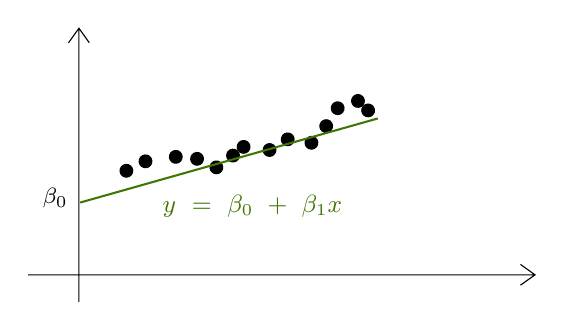
\begin{tikzpicture}[x=0.75pt,y=0.75pt,yscale=-1,xscale=1]
%uncomment if require: \path (0,195.33333206176758); %set diagram left start at 0, and has height of 195.33333206176758

%Shape: Axis 2D [id:dp35721852247943175] 
\draw  (31,131.8) -- (275.17,131.8)(55.42,13) -- (55.42,145) (268.17,126.8) -- (275.17,131.8) -- (268.17,136.8) (50.42,20) -- (55.42,13) -- (60.42,20)  ;
%Flowchart: Connector [id:dp7405838412090233] 
\draw  [fill={rgb, 255:red, 0; green, 0; blue, 0 }  ,fill opacity=1 ] (110.41,78.3) .. controls (109.09,77.23) and (108.9,75.3) .. (109.97,73.99) .. controls (111.04,72.68) and (112.96,72.49) .. (114.28,73.56) .. controls (115.59,74.62) and (115.78,76.55) .. (114.71,77.86) .. controls (113.65,79.17) and (111.72,79.37) .. (110.41,78.3) -- cycle ;
%Flowchart: Connector [id:dp4208481249614251] 
\draw  [fill={rgb, 255:red, 0; green, 0; blue, 0 }  ,fill opacity=1 ] (85.57,79.5) .. controls (84.26,78.43) and (84.06,76.5) .. (85.13,75.19) .. controls (86.2,73.88) and (88.13,73.69) .. (89.44,74.75) .. controls (90.75,75.82) and (90.95,77.75) .. (89.88,79.06) .. controls (88.81,80.37) and (86.88,80.57) .. (85.57,79.5) -- cycle ;
%Flowchart: Connector [id:dp7170407416997207] 
\draw  [fill={rgb, 255:red, 0; green, 0; blue, 0 }  ,fill opacity=1 ] (145.33,74.04) .. controls (144.02,72.97) and (143.82,71.05) .. (144.89,69.73) .. controls (145.96,68.42) and (147.89,68.23) .. (149.2,69.3) .. controls (150.51,70.36) and (150.71,72.29) .. (149.64,73.6) .. controls (148.57,74.91) and (146.64,75.11) .. (145.33,74.04) -- cycle ;
%Flowchart: Connector [id:dp9831981842904083] 
\draw  [fill={rgb, 255:red, 0; green, 0; blue, 0 }  ,fill opacity=1 ] (127.73,76.73) .. controls (126.42,75.66) and (126.22,73.73) .. (127.29,72.42) .. controls (128.36,71.11) and (130.29,70.92) .. (131.6,71.98) .. controls (132.91,73.05) and (133.1,74.98) .. (132.04,76.29) .. controls (130.97,77.6) and (129.04,77.8) .. (127.73,76.73) -- cycle ;
%Flowchart: Connector [id:dp6597419850766411] 
\draw  [fill={rgb, 255:red, 0; green, 0; blue, 0 }  ,fill opacity=1 ] (192.81,54.97) .. controls (191.5,53.9) and (191.3,51.97) .. (192.37,50.66) .. controls (193.44,49.35) and (195.37,49.15) .. (196.68,50.22) .. controls (197.99,51.29) and (198.19,53.22) .. (197.12,54.53) .. controls (196.05,55.84) and (194.12,56.04) .. (192.81,54.97) -- cycle ;
%Flowchart: Connector [id:dp12644057862139046] 
\draw  [fill={rgb, 255:red, 0; green, 0; blue, 0 }  ,fill opacity=1 ] (165.51,70.57) .. controls (164.2,69.5) and (164,67.57) .. (165.07,66.26) .. controls (166.14,64.95) and (168.07,64.75) .. (169.38,65.82) .. controls (170.69,66.89) and (170.89,68.82) .. (169.82,70.13) .. controls (168.75,71.44) and (166.82,71.63) .. (165.51,70.57) -- cycle ;
%Flowchart: Connector [id:dp9469181871169179] 
\draw  [fill={rgb, 255:red, 0; green, 0; blue, 0 }  ,fill opacity=1 ] (172.62,62.54) .. controls (171.31,61.47) and (171.11,59.54) .. (172.18,58.23) .. controls (173.25,56.92) and (175.18,56.72) .. (176.49,57.79) .. controls (177.8,58.86) and (178,60.79) .. (176.93,62.1) .. controls (175.86,63.41) and (173.93,63.6) .. (172.62,62.54) -- cycle ;
%Flowchart: Connector [id:dp7748779153505232] 
\draw  [fill={rgb, 255:red, 0; green, 0; blue, 0 }  ,fill opacity=1 ] (154.07,68.91) .. controls (152.76,67.84) and (152.57,65.91) .. (153.64,64.6) .. controls (154.71,63.29) and (156.63,63.09) .. (157.94,64.16) .. controls (159.26,65.23) and (159.45,67.16) .. (158.38,68.47) .. controls (157.31,69.78) and (155.39,69.98) .. (154.07,68.91) -- cycle ;
%Flowchart: Connector [id:dp5494330788804085] 
\draw  [fill={rgb, 255:red, 0; green, 0; blue, 0 }  ,fill opacity=1 ] (76.36,84.06) .. controls (75.05,82.99) and (74.85,81.06) .. (75.92,79.75) .. controls (76.99,78.44) and (78.92,78.25) .. (80.23,79.31) .. controls (81.54,80.38) and (81.74,82.31) .. (80.67,83.62) .. controls (79.6,84.93) and (77.67,85.13) .. (76.36,84.06) -- cycle ;
%Flowchart: Connector [id:dp5890644622068899] 
\draw  [fill={rgb, 255:red, 0; green, 0; blue, 0 }  ,fill opacity=1 ] (100.16,77.35) .. controls (98.85,76.28) and (98.65,74.35) .. (99.72,73.04) .. controls (100.79,71.73) and (102.72,71.53) .. (104.03,72.6) .. controls (105.34,73.67) and (105.53,75.6) .. (104.46,76.91) .. controls (103.4,78.22) and (101.47,78.42) .. (100.16,77.35) -- cycle ;
%Flowchart: Connector [id:dp10183370135658154] 
\draw  [fill={rgb, 255:red, 0; green, 0; blue, 0 }  ,fill opacity=1 ] (119.71,82.41) .. controls (118.4,81.35) and (118.2,79.42) .. (119.27,78.11) .. controls (120.34,76.8) and (122.27,76.6) .. (123.58,77.67) .. controls (124.89,78.74) and (125.09,80.67) .. (124.02,81.98) .. controls (122.95,83.29) and (121.02,83.48) .. (119.71,82.41) -- cycle ;
%Flowchart: Connector [id:dp13579805852853988] 
\draw  [fill={rgb, 255:red, 0; green, 0; blue, 0 }  ,fill opacity=1 ] (132.83,72.55) .. controls (131.52,71.48) and (131.32,69.55) .. (132.39,68.24) .. controls (133.46,66.93) and (135.39,66.74) .. (136.7,67.81) .. controls (138.01,68.87) and (138.2,70.8) .. (137.13,72.11) .. controls (136.07,73.42) and (134.14,73.62) .. (132.83,72.55) -- cycle ;
%Flowchart: Connector [id:dp1916741178210739] 
\draw  [fill={rgb, 255:red, 0; green, 0; blue, 0 }  ,fill opacity=1 ] (178.15,53.91) .. controls (176.84,52.84) and (176.64,50.92) .. (177.71,49.61) .. controls (178.78,48.29) and (180.71,48.1) .. (182.02,49.17) .. controls (183.33,50.24) and (183.53,52.16) .. (182.46,53.47) .. controls (181.39,54.79) and (179.46,54.98) .. (178.15,53.91) -- cycle ;
%Flowchart: Connector [id:dp17036893605725] 
\draw  [fill={rgb, 255:red, 0; green, 0; blue, 0 }  ,fill opacity=1 ] (187.94,50.41) .. controls (186.62,49.34) and (186.43,47.41) .. (187.5,46.1) .. controls (188.57,44.79) and (190.49,44.59) .. (191.8,45.66) .. controls (193.12,46.73) and (193.31,48.66) .. (192.24,49.97) .. controls (191.17,51.28) and (189.25,51.48) .. (187.94,50.41) -- cycle ;
%Straight Lines [id:da2624274909662574] 
\draw [color={rgb, 255:red, 65; green, 117; blue, 5 }  ,draw opacity=1 ][line width=0.75]    (56.05,96.98) -- (199.41,56.48) ;



% Text Node
\draw (44,95) node  [font=\footnotesize] [align=left] {$\displaystyle \beta _{0}$};
% Text Node
\draw (139,99) node  [font=\small,color={rgb, 255:red, 65; green, 117; blue, 5 }  ,opacity=1 ] [align=left] {$\displaystyle y\ =\ \beta _{0} \ +\ \beta _{1} x$};


\end{tikzpicture}
\begin{enumerate}
  \setcounter{enumi}{1}
	\item	The distance of the points to the line are the \textbf{residuals} $\varepsilon$.
	\item	When we plot the SSR for the different possible curve, we pick the one with the \textit{smallest SSR}. 
	\begin{itemize}
		\item	That is to say, we pick the one with the \textbf{Least Squares}.
		\item 	That curve is the curve such that the derivative has a slope of 0 and it becomes the \textbf{Least Squares Estimator}.
	\end{itemize}
\end{enumerate}
\end{YTB_SUMM}

\begin{YTB_SUMM}{\href{https://www.youtube.com/watch?v=2AQKmw14mHM&list=PLblh5JKOoLUIzaEkCLIUxQFjPIlapw8nU&index=10}{StatQuest: R-squared explained}}
For comprehension, we define the measure of correlation by $R$ rather than $\rho$.
\begin{enumerate}
	\item	The main idea to retain is that $R^{2}$ is a \textbf{metric of correlation}.
	\item	In fact, $R^{2}$ is literally the \textbf{correlation squared},  $R^{2} = (R)^{2}$.
	\begin{itemize}
		\item	The advantage is that it's much easier to interpret and to calculate.
		\item	It's not obvious that $R = 0.7$ is twice as good as $R = 0.5$ but $R^{2} = 0.7^{2} = 0.5$ is clearly twice as good as $R^{2} = 0.5^{2} = 0.25$.
	\end{itemize}
	\item	The same idea from the Least Squares video is used, we want the line that will minimise the SSR. Now however, we want to \textbf{quantify how good} this new \textbf{line is} and we use the $R^{2}$.
	\item	$R^{2} = \frac{\text{Var}(\text{mean}) - \text{Var}(\text{Least Squares line})}{\text{Var}(\text{mean})}$. 
	\begin{itemize}
		\item	That is to say we divide the difference in the variation of the points to the line (SSR) by the variation of the points to the line that goes through the mean;
		\item	Thereby, this has to be between 0 and 1 since the SSR for any line is $\le$ SSR for the line going through the mean;
		\item	Thus $0 \le R^{2} \le 1$ and it is a percentage.
	\end{itemize}
	\item	The interpretation of $R^{2}$ can be either:
	\begin{itemize}
		\item	There is 81\% less variation around the line than the mean;
		\item	The line explains 81\% of the variation of the relationship between the two variables.
	\end{itemize}
	\item	Thus, logically we want to maximise the $R^{2}$.
	\item	\textbf{Note}: $R^{2}$ doesn't indicate the direction of the relationship like $R$ does.
\end{enumerate}
\end{YTB_SUMM}

\begin{YTB_SUMM}{\href{https://www.youtube.com/watch?v=nk2CQITm_eo&list=PLblh5JKOoLUIzaEkCLIUxQFjPIlapw8nU&index=2}{StatQuest: Linear Models Pt.1 - Linear Regression}}
\begin{enumerate}
	\item	Reminder on $R^{2}$ 
	\begin{itemize}
		\item	Evaluates how well a line fits;
		\item	SS(mean) = (data - mean)$^{2}$: Sum of Squares around the mean ($\bar{y}$);
		\item	$\text{Var}(\text{mean}) = \frac{(\text{data} - \text{mean})^{2}}{n}$: Variation of the data around the mean ($\bar{y}$);
		\item	SS(fit) = (data - fit)$^{2}$: Sum of Squares around the fitted Least Squares line;
		\item	$\text{Var}(\text{fit}) = \frac{(\text{data} - \text{fit})^{2}}{n}$: Variation of the data around the best fit line;
		\item	In general, $\text{Var}(\text{something}) = \frac{SS(\text{something})}{\text{number of things}}$;
		\item	Thus, $R^{2} = \frac{SS(\text{mean}) - SS(\text{fit})}{SS(\text{mean})} \Leftrightarrow \frac{\text{Var}(\text{mean}) - \text{Var}(\text{fit})}{\text{Var}(\text{mean})}$.
	\end{itemize}	
	\item	Note on \textbf{adding variables}
	\begin{itemize}
		\item	More parameters will always have a "\textit{\textbf{better}}" fit because the Least Squares line will set useless variables's parameters to 0;
		\item	Thereby, the SS(fit) will decrease causing the $R^{2}$ to increase;
		\item	This is not always a good thing. For example, if we add the result of a coin flip as a variable then it is possible that by chance heavier mice will get more heads. This would mean that a nonsensical variable would lead to a better $R^{2}$;
		\item	This is why often times the adjusted $R^{2}_{a}$ is reported instead of the $R^{2}$.
	\end{itemize}		
	\item	Note on the \textbf{number of data points}
	\begin{itemize}
		\item	If, for example, there were only 2 points then the line would have a perfect fine leading to a $R^{2} = 1$.
		\item	However, this is true for any 2 points with a line connecting them.
		\item	Therefore, we want a measure of the significance of the $R^{2}$, we want a \textbf{p-value}.
	\end{itemize}
	\item	To account for the 2 problems of the \textit{number of parameters} and the \textit{amount of data}, we define $F$. 
	\begin{itemize}
		\item	First, we compare what the equations mean in text:	
\setlength{\mathindent}{-2cm}				
		\begin{align*}
			R^{2}	&=	\frac{\text{variance in size that \textbf{IS} explained by adding weight}}{\text{variance in size \textbf{WITHOUT} weight taken into account}}	\\
			F	&=	\frac{\text{variance in size that \textbf{IS} explained by adding weight}}{\text{variance in size \textbf{NOT} explained by adding weight}}	
		\end{align*}
		Thus, the denominator of $F$ is the variance of the points to the line, or, \textbf{the error} in the prediction of mouse size.
		\item	More formally, we get:
		\begin{align*}
			R^{2}	&=	\frac{SS(\text{mean}) - SS(\text{fit})}{SS(\text{mean})}	\\
			F	&=	\frac{\left(SS(\text{mean}) - SS(\text{fit})\right)/\left(p_{\text{fit}} - p_{\text{mean}}\right)}{SS(\text{fit})/\left(n - p_{\text{fit}}\right)}
	\end{align*}
\setlength{\mathindent}{1cm}
		\item	$\left(p_{\text{fit}} - p_{\text{mean}}\right)$ is the difference in parameters between the 2 lines; i.e., the number of parameters in addition to the y-intercept.
		\item	$\left(n - p_{\text{fit}}\right)$ is the number of observations minus the number of parameters.
		\item	These 2 are the \textbf{degrees of freedom} for the $F$ distribution.		
	\end{itemize}
	\item	Recall the \textbf{histogram of} the blocks of the $F$ values for many random samples.
	\begin{itemize}
		\item	The p-value is obtained from the $F$ distribution and is: 
		$\frac{\text{number of blocks that are just as, if not more, extreme than the block for the fitted line}}{\text{the total number of blocks from all the simulations}}$;
		\item	In practice this is \textbf{approximated with a curve} where the \textbf{degrees of freedom} are the \textbf{shape parameters}.
		\item	We note that as the \textbf{number of points goes up}, the tail tapers off (light-tailed) and thus the \textbf{p-value gets smaller}.
		\item	This makes sense as the approximation gets closer to reality, the result is more credible and thereby more significant.
	\end{itemize}	
\end{enumerate}
\end{YTB_SUMM}

\begin{YTB_SUMM}{\href{https://www.youtube.com/watch?v=zITIFTsivN8&list=PLblh5JKOoLUIzaEkCLIUxQFjPIlapw8nU&index=5}{StatQuest: Linear Models Pt.1.5 - Multiple Regression}}
	\begin{enumerate}
		\item	Same thing as simple linear regression but with more parameters.
		\item	$R^{2}$ is the same but $p_{\text{fit}}$ will increase as $p_{\text{mean}}$ stays equal to 1.
		\item	In both cases, this would be comparing the model (simple or multiple regression) to the mean but we can compare them to each other!
		\begin{itemize}
			\item	If want to know whether the addition of a second parameter, say tail length, is worth the time and effort it'll take to collect it's data we do a \textbf{partial $F$ test}:
			\begin{equation*}
				F	=	\frac{SS(\text{simple}) - SS(\text{multiple})/\left(   p_{\text{multiple}} - p_{\text{simple}} \right)}{SS(\text{multiple}) / \left( n - p_{\text{multiple}}\right)}
			\end{equation*}
		\end{itemize}
	\end{enumerate}
\end{YTB_SUMM}

\begin{YTB_SUMM}{\href{https://www.youtube.com/watch?v=NF5_btOaCig&list=PLblh5JKOoLUIzaEkCLIUxQFjPIlapw8nU&index=6}{StatQuest: Linear Models Pt.2 - t-tests and ANOVA}}
\begin{enumerate}
	\item	The \textbf{goal} of a t-test is to \textbf{compare means} and see if there's a \textbf{significant difference} between them.
	\item	General steps to a t-test are the following (while visualising a t-test and simple linear regression side-by-side):
	\begin{enumerate}
		\item	Ignore x-axis and find the overall mean
		\item	Calculate the SS(mean) for both the t-test and regression
		\item	Fit a line (we care about the x-axis now). Recall that the t-test is two lines:
		\begin{itemize}
			\item	Use indicator variables represented by a \textbf{design matrix} which has 1's for the first group and 0's for the other, and vice-versa for all observations.
			\item	The equation becomes $y = \text{column 1} \mu_{1} + \text{column 2} \mu_{2}$.
		\end{itemize}
		\item	Calculate F now that the SS(mean) and SS(fit) is found.
		\begin{itemize}
			\item	Note that $p_{\text{mean}} = 1$ because there is only the intercept as an argument.
			\item	$p_{\text{fit}} = 2$ because of the 2 indicator variables for t-test and the 2 parameters for regression.
		\end{itemize}
	\item	\textbf{ANOVA} is a generalization with more than just 2 groups' means to compare.
	\begin{itemize}
		\item	$p_{\text{mean}} = 1$ like before.
		\item	$p_{\text{fit}}$ is the number of groups / the number of parameters; 5 in the example.
		\item	Note that the design matrix can be rewritten with a column of 1's and is usally seen that way.
	\end{itemize}
	\end{enumerate}
\end{enumerate}
\end{YTB_SUMM}

\begin{YTB_SUMM}{\href{https://www.youtube.com/watch?v=CqLGvwi-5Pc&list=PLblh5JKOoLUIzaEkCLIUxQFjPIlapw8nU&index=7}{StatQuest: Linear Models Pt.3 - Design Matrices}}
\begin{enumerate}
	\item	Plus in one row at a time
	\item	Idea of 2 lines and predicted value will be on one or the other depending on the indicator variable.
	\item	Idea of comparing to the mean \textit{or} a simpler model
\end{enumerate}
\end{YTB_SUMM}

\section{Validation, sélection et qualité d'ajustement}

\subsubsection{Résumés des chapitres}

\begin{CHPT_SUMM}{5. Linear Regression:  Validation}
\begin{enumerate}
	\item	Validating model assumptions
	\begin{itemize}
		\item	Matrice chapeau $\bm{H}$ et leverage $h_{ii}$
		\item	Variance des résidus
		\item	Types de résidus
		\begin{itemize}
			\item	Résidus (raw);
			\item	Résidus standardisés;
			\item	Résidus studentisés.
		\end{itemize}
		\item	Postulats appliqués à la variable réponse
		\begin{enumerate}
			\item	Linéarité -> vérifié avec un QQplot;
			\item	Normalité -> vérifé avec un graphique des résidus $\hat{\varepsilon}$ contre les prévisions $\hat{Y}$;
			\item	Homoscédasticité -> vérifiés avec un graphique des résidus contre chaque variable explicative qui ne devrait pas avoir de tendance (\textbf{pattern}) discernable (par exemple, quadratique);
			\item	Indépendance des observations -> vérifiés avec la même graphique mais dans un ordre dont la corrélation est attendue (par exemple, si données chronologiques selon le temps).
		\end{enumerate}
	\end{itemize}
	\item	Outliers and influential points
	\begin{itemize}
		\item	2 types d'observations différents \textbf{(voir vidéos)}:
		\begin{enumerate}
			\item	\textbf{Outliers}: espacés horizontalement et détectable par un \textbf{résidu élevé}.
			\item	\textbf{Leverage points}: espacés verticalement et détectable par un \textbf{high leverage}; cependant, pas nécessairement mauvais.
		\end{enumerate}
		\item	De plus, il y a des \textbf{influential points} (les mauvais leverage points).
		\item	\textbf{Cook's distance} pour mesurer l'impact global sur les estimations des paramètres lorsque l'on retire chaque observation une à la fois.
	\end{itemize}
	\item	Collinearity of explanatory variables; VIF
	\begin{itemize}
		\item	Calcul du VIF$_{j}$ et du $R^{2}_{(j)}$;
		\item	Relation avec l'écart-type estimé du paramètre $\hat\beta_{j}$.
	\end{itemize}
\end{enumerate}
\textbf{Note sur les exercices:} 
\begin{enumerate}
	\item	Généralement peu d'exercices des examens.
	\begin{itemize}
		\item	Des exercices des examens, quelques choix multiples dont il faut dire quels affirmations sont vrai/faux de graphiques;
		\item	Important est surtout de bien saisir les concepts et savoir les différentes formulations pour les équations (Cooks' Distance, VIF / $s_{b_{j}}$, 		$\dots$).
	\end{itemize}
	\item	Exercices de \textbf{résidus} aucune question d'examen, mais semble plus logique que ce soit englobé par une question plus générale.
	\item	Exercices de \textbf{influential points}	:
	\begin{itemize}
		\item	une question d'examen;
		\item	Faire des relations des différents formules pour les trouver à partir d'info partielle.
	\end{itemize}
	\item	Exercices sur le \textbf{VIF}
	\begin{itemize}
		\item	Bien saisir le concept de faire une régression sur une autre variable explicative;
		\item	Savoir la lien entre VIF et $s_{b_{j}}$;
		\item	Savoir ce que représente $s_{x_{j}}$ et bien saisir.
	\end{itemize}
\end{enumerate}
\end{CHPT_SUMM}

\begin{CHPT_SUMM}{6. Resampling methods}
\begin{enumerate}
	\item	Les méthodes classiques statistiques posent, et testent, des hypothèses.
	\begin{itemize}
		\item	Cependant, ces méthodes sont seulement valides pour des modèles de régression linéaire.
	\end{itemize}
	\item	Les méthodes modernes utilisent la technologie pour directement évaluer la qualité des prévisions d'un modèle avec le MSE.
	\begin{itemize}
		\item	Ces méthodes sont valides pour tous les modèles;
		\item	Le livre rappelle la balance entre la variance et le biais pour le MSE.
	\end{itemize}
	\item	La problématique principale est que si l'on utilise toutes les données pour établir le modèle on ne peut pas le tester. Le chapitre couvre donc 2 méthodes de séparer les données pour les tester:
	\begin{enumerate}
		\item	\textbf{Validation set approach}: On partitionne aléatoirement l'ensemble de données en 1 ensemble d'entrainement et un ensemble de validation.
		\begin{itemize}
			\item	Habituellement, l'ensemble de validation comporte entre 25 et 35\% des données;
			\item	Un désavantage est que le modèle est ajusté sur seulement une partie des données et donc la variabilité des résultats augmente et le MSE sera une sur-estimation du vrai MSE;
			\item	Un autre désavantage est que puisque la séparation est aléatoire, le MSE peut être très variable.
		\end{itemize}
		\item	\textbf{Cross-validation}: Partitionne les données systématiquement et prends la moyenne des MSE des sous-ensembles. 2 méthodes sont abordées:
		\begin{enumerate}
			\item	\textbf{Leave One Out Cross Validation (LOOCV)}: Ajuste le modèle en excluant une observation à la fois pour toutes les observations et en prends la moyenne.
			\item	\textbf{k-fold Cross Validation}: Partitionne les données en k sous-ensembles et en prends la moyenne.
		\end{enumerate}
	\end{enumerate}
	\item	Le livre explique les pros/cons des différentes méthodes.
\end{enumerate}
\textbf{Note sur les exercices:} 
\begin{enumerate}
	\item	Savoir différents statistiques pour out of sample et la validation croisée;
	\item	Savoir le lien entre k-fold et LOOOCV et le lien avec la variance/biais.
\end{enumerate}
\end{CHPT_SUMM}

\begin{CHPT_SUMM}{7. Linear Regression:  Subset Selection}
L'importance de la section est surtout de comprendre que puisque l'ajustement sera toujours \textit{meilleur} avec plus de paramètres, nous devons établir des méthodes de réduire le nombre de paramètres. 

S'il y a $p$ paramètres, alors il y a $2^{p}$ possibilités de modèles. Il est donc important de comprendre qu'on ne peut pas tester autant de possibilités de modèles et donc qu'on doit établir des méthodes de sélection de modèle algorithmique.

Finalement, on veut comparer des différents modèles et c'est de là que vient les différentes statistiques de comparaison de modèles qui prennent en compte le nombre de paramètres $p$ ainsi que l'ajustement du modèle $SS(\text{résidus})$.

\begin{enumerate}
	\item	Sélection de sous-ensembles
	\begin{itemize}
		\item	Les deux méthodes les mieux connues sont la sélection \textbf{backward} et la sélection \textbf{forward};
		\item	Il faut savoir non seulement leurs algorithmes, mais comprendre qu'ils font partie de l'approche \textbf{stepwise};
		\item	Faut savoir et comprendre le nombre de modèles possible maximal;
		\item	Faut savoir et comprendre que ces méthodes ne garantie pas le meilleur modèle;
		\item	Faut savoir la \textbf{mixed method} qui est en réalité assez semblable à faire des drop1;
		\item	Lire et comprendre les différents problèmes.
	\end{itemize}
	\item	Sélection du meilleur modèle
	\begin{itemize}
		\item	La validation croisée est la plus précise mais nécessite beaucoup de computing power;
		\item	La pénalité qu'on applique avec les diverses statistiques servent à estimer l'inflation du MSE en comparaison au vrai MSE;
		\item	Lire et savoir les différentes formules pour l'AIC, BIC, $C_{p}$ de Mallow, $R^{2}_{a}$;
		\item	Comprendre que la pénalité du BIC est supérieur à celle de l'AIC et donc qu'il aura tendance à conserver moins de paramètres.s
	\end{itemize}
\end{enumerate}
\textbf{Note sur les exercices:} Généralement 5 types
\begin{enumerate}
	\item	Déterminer le nombre de possibilités de modèles selon les différents algorithmes stepwise;
	\item	Sélectionner un modèle selon stepwise;
	\item	Calculer / isoler le $C_{p}$ de Mallows;
	\item	Calculer / isoler le $C_{a}^{2}$.
\end{enumerate}
\end{CHPT_SUMM}

\begin{CHPT_SUMM}{8. Linear Regression:  Shrinkage and Dimension Reduction}
\begin{enumerate}
	\item	\textbf{Shrinkage methods}: On fait la sélection de variables soit en réduisant les coefficients ou en les retirant.
	\begin{itemize}
		\item	Régression \textbf{Ridge}: utile pour la multicolinéarité en réduisant des coefficients;
		\item	Régression \textbf{Lasso}: utile pour la sélection de variables en posant des coefficients égale à 0;
		\item	Dans les deux cas, on trouve la balance entre l'augmentation du biais et la diminution de la variance où le MSE est minimisé;
		\item	Nous avons soit le \textbf{tuning parameter} $\lambda$ ou le \textbf{budget alloué} \textbf{s}.
	\end{itemize}
	\item	\textbf{Méthodes de réduction de dimensions}: \textbf{Au lieu} de \textit{\textbf{réduire}} le nombre de variables nécessaire pour le modèle, on \textbf{\textit{crée}} des \textbf{nouvelles variables} qui sont des \textbf{combinaisons linéaires} des variables originales.
	\item[]	Deux méthodes abordées: 
	\begin{enumerate}
		\item	\textbf{Principal Components Regression}: méthode \textit{non-supervisée} (sans variable réponse) d'\textbf{identifier les variables} pour lesquelles les données sont \textbf{le plus variable};
		\item[]	\textbf{Note}: Ceci est principalement couvert au \textbf{chapitre 17}, et on ne devrait pas vraiment s'attendre à le comprendre ici.
		\begin{itemize}
%			\item	Pour sélectionner le \textbf{principal component} $Z_{1} = \sum_{j} \phi_{j1} X_{j}$, on fait la sélection des $\phi_{j1}$ t.q. $\sum \phi^{2}_{j1} = 1$ et la variance de $\sum_{j = 1}^{k} \phi_{j1}(X_{j} - \bar{X}_{j})$ est maximisée. Sa direction est celle minimisant l'écart entre la ligne et les données;
%			\item	Le deuxième \textbf{principal component} est choisit tel qu'il n'est pas corrélé au premier et que la variance est maximisée. Sa direction est perpendiculaire au premier;
%			\item	Les vecteurs $Z_{i}$ ont $n$ composantes (comme les $X_{i}$). Par exemple, les composantes de $Z_{1}$ sont $z_{i1} = \sum_{j = 1}^{k}\phi_{j1}(x_{ij} - \bar{x_{j}})$;
			\item	Les $\phi_{ji}$ sont surnommés les \textbf{loadings} et les $z_{i1}$ les \textbf{principal component scores};
			\item	Les \textit{scores} sont la distance entre les points et les \textit{principal components};
			\item	La \textbf{régression} de principal components (PCR) est \textbf{sur les principal components};
			\item	Puisqu'ils sont des moyennes pondérées de toutes les variables, PCR ne \textbf{fait pas la sélection de variable} et est semblable à la régression ridge dans ce sens;
			\item	Le plus de composantes, le plus faible le biais et le plus élevé la variance.
		\end{itemize}
		\item	\textbf{Partial Least Squares}: méthode \textit{supervisée};
		\begin{itemize}
			\item	Puisque la variable réponse est prise en compte, la direction n'est pas aussi bien ajusté;
			\item	Les prédicteurs cependant seront mieux à expliquer la réponse;
			\item	Réduit le biais en comparaison au PCA, mais augmente la variance et donc n'est pas globalement supérieur au PCA.
		\end{itemize}
	\end{enumerate}
	\item	\textbf{The curse of dimensionality}: Adding variables to a model with many variables will cause the model to deteriorate, unless the variables are truly related to the response.
	\begin{itemize}
		\item	Si le nombre de variable est large, particulièrement si $p \ge n$, l'ajustement sera parfait met les coefficients seront mal-définis;
		\item	Donc, les statistiques vont indiquer un superbe modèle alors qu'en réalité il va très mal performer.
	\end{itemize}
\end{enumerate}
\textbf{Note sur les exercices:} Généralement soit:
\begin{enumerate}
	\item	Questions qualitatives
	\begin{itemize}
		\item	Les questions d'exam semblaient être  +/- juste ça;
		\item	Bien saisir le lien avec le SSE et les différentes méthodes de régression;
		\item	Savoir et comprendre le lien entre le budget alloué $s$ et $\lambda$;
		\item	Savoir et comprendre la distinction entre PCA et PLS.
	\end{itemize}
	\item	Questions quantitatives
	\begin{itemize}
		\item	Les questions les plus semblable à ce qui pourrait être dans l'exam je crois que ce serait comme 8.14 ou 8.3/8.8, le reste j'ai vraiment l'impression que c'est plus pour qu'on saisit les concepts.
	\end{itemize}
\end{enumerate}
\end{CHPT_SUMM}

\subsubsection{Notes sur les vidéos YouTube}

\begin{YTB_SUMM}{\href{https://www.youtube.com/watch?v=Z-jXJpVohiI}{Phil Chan: Introduction to the Hat matrix in regression}}
It is essential to visualize the plane from the video.
\begin{enumerate}
	\item	$\matr{H}$ is a function of the explanatory variables; $\matr{H} = \matr{X(X^{\top}X)^{-1}X^{\top}}$.
	\begin{itemize}
		\item	It is called the \textbf{hat} matrix;
		\item	It is an \textbf{orthogonal} \textbf{projection} matrix that \og \textit{maps a vector into the column space spanned by $\bm{X}$} \fg{}.
	\end{itemize}
	\item	It is called the \textbf{Hat} matrix because it puts a \textit{hat} on $\bm{Y}$; $\matr{\hat{Y} = H Y}$.
	\begin{itemize}
		\item	The proof for this consists of realizing we can isolate $\bm{\hat{\beta}}$ in the formula.
	\end{itemize}
	\item	It is an \textbf{orthogonal} matrix because it picks the point on the plane (column space) closest to the real observation. By definition, that will be the point directly below the value. That is to say, the \textit{\textbf{orthogonal}} point.
	\item	The project matrix $\matr{I - H = M}$ maps the plan orthogonal to the previous one. That is to say, the space between the observation and the original plane.
	\begin{itemize}
		\item	Doing this, we can visually see that $\matr{Y = HY + MY}$.
	\end{itemize}
\end{enumerate}
\end{YTB_SUMM}

\begin{YTB_SUMM}{\href{https://www.youtube.com/watch?v=l2xG_yehq0k&t=146s}{Phil Chan: How is it the Hat matrix spans the column space of X? Really nice.}}
This video explains why the hat matrix is what it is from a different angle which really helps to better understand.
\begin{enumerate}
	\item	$\bm{H}$ is a \textit{projection matrix} of a vector (which is a function of $\bm{X}$) onto a column space.
	\begin{itemize}
	\item	Visualise the $H = (v_1 \ v_2  \ \dots \ v_n)$ where there are bars above and below the $v_{i}$s to exemplify \textit{span}.	
	\end{itemize}
	\item	We want to get $\bm{\hat{\beta}}$ from the equation $\matr{Y = X }\bm{\hat{\beta}}$ but we can't just inverse $\bm{X}$.
	\begin{itemize}
		\item	If $\bm{X}$ were square that would mean that there would be as many observations as parameters ($n = p$);
		\item	If $\bm{Y}$ were \og \textit{on the same column space as $\bm{X}$} \fg{} then $\bm{Y}$ would be on the same plane as $\bm{X}$ which is of course almost never the case;
		\item	This is why we have $\bm{\hat{Y}}$ \textit{which \textbf{is}} on the column space of $\bm{X}$;
		\item	Finally, we recall from the previous video that that point will have to be \textit{orthogonal} to $\bm{Y}$ and deduce that distance \textbf{must be $\matr{Y - \hat{Y} = Y - X} \bm{\hat{\beta}}$}.
	\end{itemize}
	\item	The next step is to realize the inner product of the observations to this vector must be zero and therefore that $\matr{X^{\top}(Y - \hat{Y})} = 0$.
	\begin{itemize}
		\item	Finally we isolate this to find $\matr{\hat{\beta} = X(X^{\top}X)^{-1}X^{\top}Y}$ which means $\bm{H}$ must be $\matr{(X^{\top}X)^{-1}X^{\top}}$.
	\end{itemize}
\end{enumerate}
\end{YTB_SUMM}

\begin{YTB_SUMM}{\href{https://www.youtube.com/watch?v=UyAa5iwJ7m0&list=PLe0nS0mZ7vGGhYcDPNSVNu9gT3wGHbjhu&index=3}{Phil Chan: Should I look at raw, standardized, or studentized residuals? part 1 - what to look out for}}
\begin{enumerate}
	\item	The (raw) residual $\hat\varepsilon_{i} = \text{observation}_{i} - \text{predicted}_{i}$.
	\item	Want the graphics to be random.
	\begin{itemize}
		\item	If there are far points that could suggest outliers;
		\item	If there is a pattern with the points (for example quadratic) that could suggest a non-linear relationship / collinearity;
		\item	If there is a pattern with the points and we plot it against time that could suggest (auto)correlation;
		\item	If there is an irregular variance that could suggest heteroscedasticity.
	\end{itemize}
	\item	Moral of the story, better with either the studentised or standardised residuals than the raw residuals.
\end{enumerate}
\end{YTB_SUMM}

\begin{YTB_SUMM}{\href{https://www.youtube.com/watch?v=UyAa5iwJ7m0&list=PLe0nS0mZ7vGGhYcDPNSVNu9gT3wGHbjhu&index=4}{Phil Chan: Should I look at raw, standardized, or studentized residuals? part 2 - kinds of residuals}}
There are 2 main problems that explain why we use the standardised or studentised residuals instead of the raw residuals:
\begin{enumerate}
	\item	The \textbf{heteroscedasticity} assumption \textbf{\textit{doesn't} mean} the \textbf{variance} will be the \textbf{same for all (raw) residuals}.
	\begin{itemize}
		\item	If that were true, we'd have a horizontal line for the (raw) residuals which is never the case.
		\item	The reality is thus that some (raw) residuals' variance will be larger than others'.
	\end{itemize}
	\item	The (raw) \textbf{residuals} are \textbf{measured} in the \textbf{same units} \textbf{as the observations}.
	\begin{itemize}
		\item	In case this doesn't make sense, recall that $\matr{\hat{\varepsilon} = Y - \hat{Y}}$.
		\item	For example, they could range from -60000 to 340000 and thus it's hard to know whether that's good or bad.
		\item	It also makes it difficult to compare the (raw) residuals of different models.
	\end{itemize}
	\item	Thus we transform them by reducing by the mean and standardising by the standard deviation; that is to say, a \textbf{standard normal distribution}.
	\begin{itemize}
		\item	It is interesting to note that the 3 residuals (raw, standardised, and studentised) will all look similar but have a different y-axis.
		\item	With the transformation, this means that variance will be $\approx 1$ because we've converted it into a standard normal distribution.
		\item	The intuition for the general rule that we want the residuals to be between -3 and 3 is that 99.7\% of observations will be within 3 standard deviations of the mean. That is to say, $3 \sigma = 3 (1)$.
		\item	Therefore, \textbf{we can} still have some observations outside this range however it doesn't necessarily mean they're outliers. We should be concerned only if there are several.
	\end{itemize}
\end{enumerate}
\end{YTB_SUMM}

\begin{YTB_SUMM}{\href{https://www.youtube.com/watch?v=mEdSj3wlN4Q}{Phil Chan: Should I look at raw, standardized, or studentized residuals? part 3}}
Recall the formula $\text{Var}(\hat{\varepsilon}_{i}) = \sigma^{2}(1 - h_{ii})$ with $1/n \le h_{ii} \le 1$.

$h_{ii}$ is the \textbf{leverage} of point $i$. 
\begin{enumerate}
	\item	If $h_{ii}$ were the same for all observations, then the variance would be constant but this is not realistic.
	\item	The problem in finding the variance is not with $h_{ii}$, which is a \textbf{function of the observations}, but rather in finding the \textbf{unknown} variance of the error term $\sigma^{2} = \text{Var}(\varepsilon_{i})$.
	\item	The difference between the standardised and studentised residuals is thus the estimation of $\sigma^{2}$.
	\begin{itemize}
		\item	For the standardised residuals, $\sigma^{2} = s^{2} = \frac{\text{SSE}}{n - p'}$;
		\item	For the studentised residuals, we estimate the model with the $i^{\text{th}}$ observation excluded and obtain the variance of the error term $\sigma^{2}_{(i)}$ the same way \textbf{with the \textit{new} model}.
	\end{itemize}
	\item	It is important to understand that the variation of the residuals $\text{Var}(\hat{\varepsilon})$ can come from \textbf{either of} the 2 components of the formula. 
	\begin{itemize}
		\item	Visually, it is hard to differentiate which one is causing the variance; 
		\item	For heteroscedasticity verification however, we're interested in the variance of the error term $\sigma^{2}$.
	\end{itemize}
\end{enumerate}
\end{YTB_SUMM}

\begin{YTB_SUMM}{\href{https://www.youtube.com/watch?v=s5X_Poq9dJA}{Phil Chan: What's the difference between an outlier and a leverage point in regression?}}
The graph below has a mass of points with an outlier (point A) and two leverage points (B and C):

\tikzset{every picture/.style={line width=0.75pt}} %set default line width to 0.75pt        
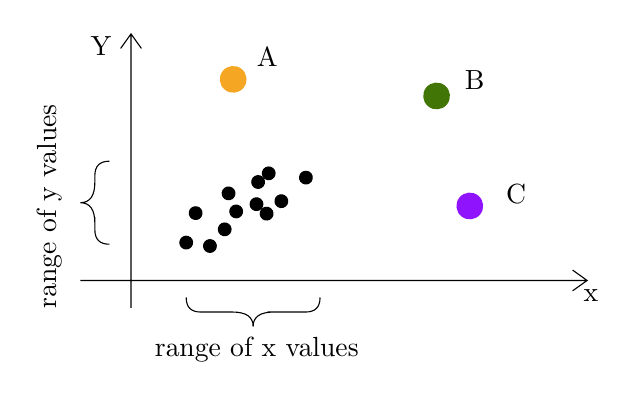
\begin{tikzpicture}[x=0.75pt,y=0.75pt,yscale=-1,xscale=1]
%uncomment if require: \path (0,195.33333206176758); %set diagram left start at 0, and has height of 195.33333206176758

%Shape: Axis 2D [id:dp9794330225749337] 
\draw  (31,131.8) -- (275.17,131.8)(55.42,13) -- (55.42,145) (268.17,126.8) -- (275.17,131.8) -- (268.17,136.8) (50.42,20) -- (55.42,13) -- (60.42,20)  ;
%Flowchart: Connector [id:dp830729222821748] 
\draw  [fill={rgb, 255:red, 0; green, 0; blue, 0 }  ,fill opacity=1 ] (114.73,86.73) .. controls (113.42,85.66) and (113.22,83.73) .. (114.29,82.42) .. controls (115.36,81.11) and (117.29,80.92) .. (118.6,81.98) .. controls (119.91,83.05) and (120.1,84.98) .. (119.04,86.29) .. controls (117.97,87.6) and (116.04,87.8) .. (114.73,86.73) -- cycle ;
%Flowchart: Connector [id:dp6451039498288915] 
\draw  [fill={rgb, 255:red, 0; green, 0; blue, 0 }  ,fill opacity=1 ] (118.81,101.97) .. controls (117.5,100.9) and (117.3,98.97) .. (118.37,97.66) .. controls (119.44,96.35) and (121.37,96.15) .. (122.68,97.22) .. controls (123.99,98.29) and (124.19,100.22) .. (123.12,101.53) .. controls (122.05,102.84) and (120.12,103.04) .. (118.81,101.97) -- cycle ;
%Flowchart: Connector [id:dp8011172696007964] 
\draw  [fill={rgb, 255:red, 0; green, 0; blue, 0 }  ,fill opacity=1 ] (91.51,117.57) .. controls (90.2,116.5) and (90,114.57) .. (91.07,113.26) .. controls (92.14,111.95) and (94.07,111.75) .. (95.38,112.82) .. controls (96.69,113.89) and (96.89,115.82) .. (95.82,117.13) .. controls (94.75,118.44) and (92.82,118.63) .. (91.51,117.57) -- cycle ;
%Flowchart: Connector [id:dp8507144087849559] 
\draw  [fill={rgb, 255:red, 0; green, 0; blue, 0 }  ,fill opacity=1 ] (98.62,109.54) .. controls (97.31,108.47) and (97.11,106.54) .. (98.18,105.23) .. controls (99.25,103.92) and (101.18,103.72) .. (102.49,104.79) .. controls (103.8,105.86) and (104,107.79) .. (102.93,109.1) .. controls (101.86,110.41) and (99.93,110.6) .. (98.62,109.54) -- cycle ;
%Flowchart: Connector [id:dp928443309589182] 
\draw  [fill={rgb, 255:red, 0; green, 0; blue, 0 }  ,fill opacity=1 ] (80.07,115.91) .. controls (78.76,114.84) and (78.57,112.91) .. (79.64,111.6) .. controls (80.71,110.29) and (82.63,110.09) .. (83.94,111.16) .. controls (85.26,112.23) and (85.45,114.16) .. (84.38,115.47) .. controls (83.31,116.78) and (81.39,116.98) .. (80.07,115.91) -- cycle ;
%Flowchart: Connector [id:dp894085737436997] 
\draw  [fill={rgb, 255:red, 0; green, 0; blue, 0 }  ,fill opacity=1 ] (119.83,82.55) .. controls (118.52,81.48) and (118.32,79.55) .. (119.39,78.24) .. controls (120.46,76.93) and (122.39,76.74) .. (123.7,77.81) .. controls (125.01,78.87) and (125.2,80.8) .. (124.13,82.11) .. controls (123.07,83.42) and (121.14,83.62) .. (119.83,82.55) -- cycle ;
%Flowchart: Connector [id:dp3127096830825926] 
\draw  [fill={rgb, 255:red, 0; green, 0; blue, 0 }  ,fill opacity=1 ] (104.15,100.91) .. controls (102.84,99.84) and (102.64,97.92) .. (103.71,96.61) .. controls (104.78,95.29) and (106.71,95.1) .. (108.02,96.17) .. controls (109.33,97.24) and (109.53,99.16) .. (108.46,100.47) .. controls (107.39,101.79) and (105.46,101.98) .. (104.15,100.91) -- cycle ;
%Flowchart: Connector [id:dp6496496287297344] 
\draw  [fill={rgb, 255:red, 0; green, 0; blue, 0 }  ,fill opacity=1 ] (113.94,97.41) .. controls (112.62,96.34) and (112.43,94.41) .. (113.5,93.1) .. controls (114.57,91.79) and (116.49,91.59) .. (117.8,92.66) .. controls (119.12,93.73) and (119.31,95.66) .. (118.24,96.97) .. controls (117.17,98.28) and (115.25,98.48) .. (113.94,97.41) -- cycle ;
%Flowchart: Connector [id:dp37437672154336576] 
\draw  [fill={rgb, 255:red, 0; green, 0; blue, 0 }  ,fill opacity=1 ] (104.04,87.25) .. controls (105.47,88.15) and (105.9,90.04) .. (105,91.47) .. controls (104.09,92.9) and (102.2,93.33) .. (100.77,92.42) .. controls (99.34,91.52) and (98.92,89.63) .. (99.82,88.2) .. controls (100.72,86.77) and (102.61,86.34) .. (104.04,87.25) -- cycle ;
%Flowchart: Connector [id:dp2062562321723702] 
\draw  [fill={rgb, 255:red, 0; green, 0; blue, 0 }  ,fill opacity=1 ] (88.19,96.75) .. controls (89.62,97.65) and (90.05,99.54) .. (89.14,100.97) .. controls (88.24,102.4) and (86.35,102.83) .. (84.92,101.92) .. controls (83.49,101.02) and (83.06,99.13) .. (83.96,97.7) .. controls (84.87,96.27) and (86.76,95.84) .. (88.19,96.75) -- cycle ;
%Flowchart: Connector [id:dp6022505758892014] 
\draw  [fill={rgb, 255:red, 0; green, 0; blue, 0 }  ,fill opacity=1 ] (141.32,79.64) .. controls (142.75,80.54) and (143.18,82.43) .. (142.27,83.86) .. controls (141.37,85.29) and (139.48,85.72) .. (138.05,84.81) .. controls (136.62,83.91) and (136.19,82.02) .. (137.09,80.59) .. controls (138,79.16) and (139.89,78.73) .. (141.32,79.64) -- cycle ;
%Flowchart: Connector [id:dp45176419201286167] 
\draw  [fill={rgb, 255:red, 0; green, 0; blue, 0 }  ,fill opacity=1 ] (129.48,91.01) .. controls (130.91,91.91) and (131.34,93.8) .. (130.44,95.23) .. controls (129.54,96.66) and (127.64,97.09) .. (126.21,96.19) .. controls (124.78,95.28) and (124.36,93.39) .. (125.26,91.96) .. controls (126.16,90.53) and (128.05,90.1) .. (129.48,91.01) -- cycle ;
%Flowchart: Connector [id:dp8281323481872875] 
\draw  [draw opacity=0][fill={rgb, 255:red, 65; green, 117; blue, 5 }  ,fill opacity=1 ] (206.71,37.91) .. controls (203.96,35.66) and (199.9,36.07) .. (197.65,38.83) .. controls (195.4,41.59) and (195.81,45.64) .. (198.57,47.89) .. controls (201.33,50.14) and (205.39,49.73) .. (207.63,46.97) .. controls (209.88,44.21) and (209.47,40.16) .. (206.71,37.91) -- cycle ;
%Flowchart: Connector [id:dp37135050597913954] 
\draw  [draw opacity=0][fill={rgb, 255:red, 144; green, 19; blue, 254 }  ,fill opacity=1 ] (222.71,90.91) .. controls (219.96,88.66) and (215.9,89.07) .. (213.65,91.83) .. controls (211.4,94.59) and (211.81,98.64) .. (214.57,100.89) .. controls (217.33,103.14) and (221.39,102.73) .. (223.63,99.97) .. controls (225.88,97.21) and (225.47,93.16) .. (222.71,90.91) -- cycle ;
%Flowchart: Connector [id:dp6196495516071849] 
\draw  [draw opacity=0][fill={rgb, 255:red, 245; green, 166; blue, 35 }  ,fill opacity=1 ] (108.71,29.91) .. controls (105.96,27.66) and (101.9,28.07) .. (99.65,30.83) .. controls (97.4,33.59) and (97.81,37.64) .. (100.57,39.89) .. controls (103.33,42.14) and (107.39,41.73) .. (109.63,38.97) .. controls (111.88,36.21) and (111.47,32.16) .. (108.71,29.91) -- cycle ;
%Shape: Brace [id:dp8715697539003557] 
\draw   (82,140) .. controls (82,144.67) and (84.33,147) .. (89,147) -- (104.25,147) .. controls (110.92,147) and (114.25,149.33) .. (114.25,154) .. controls (114.25,149.33) and (117.58,147) .. (124.25,147)(121.25,147) -- (139.5,147) .. controls (144.17,147) and (146.5,144.67) .. (146.5,140) ;
%Shape: Brace [id:dp457515066568027] 
\draw   (45,74.33) .. controls (40.33,74.33) and (38,76.66) .. (38,81.33) -- (38,84.33) .. controls (38,91) and (35.67,94.33) .. (31,94.33) .. controls (35.67,94.33) and (38,97.66) .. (38,104.33)(38,101.33) -- (38,107.33) .. controls (38,112) and (40.33,114.33) .. (45,114.33) ;

% Text Node
\draw (121,24) node   [align=left] {A};
% Text Node
\draw (221,35) node   [align=left] {B};
% Text Node
\draw (241,90) node   [align=left] {C};
% Text Node
\draw (116,165) node   [align=left] {range of x values};
% Text Node
\draw (277,139) node   [align=left] {x};
% Text Node
\draw (41,19) node   [align=left] {Y};
% Text Node
\draw (16,96) node  [rotate=-270] [align=left] {range of y values};

\end{tikzpicture}
\begin{enumerate}
	\item	To understand the difference between \textbf{outliers} and \textbf{leverage points} it is important to compare them to the mass of points and \textbf{\textit{not} the regression line}.
	\item	Outliers are points which are away from the main mass of points in the y direction (vertically).
	\begin{itemize}
		\item	When we \textit{then} add the regression line, we see this means that \textbf{outliers have a large residual}.
	\end{itemize}
	\item	Leverage points are away from the main mass of points in the x direction (horizontally).
	\begin{itemize}
		\item	There is a distinction to make between "\textit{good}" and "\textit{bad}" leverage points.
		\item	Visually, if we drew a line we can see that B is not too far out of the direction it would have whilst C is.
		\begin{itemize}
			\item	"\textit{good}" leverage points won't "damage" the model, i.e. influence the line's direction, too much.
			\item	"\textit{bad}" leverage points will. For example, C would drag the line down; it would be an \textbf{influential point}.
		\end{itemize}
		\item	To visualise, we can imagine a see-saw with C dragging down the main mass a bit:
	\end{itemize}

\tikzset{every picture/.style={line width=0.75pt}} %set default line width to 0.75pt        

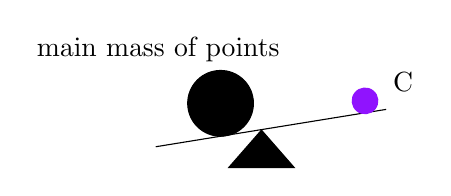
\begin{tikzpicture}[x=0.75pt,y=0.75pt,yscale=-1,xscale=1]
%uncomment if require: \path (0,195.33333206176758); %set diagram left start at 0, and has height of 195.33333206176758

%Shape: Triangle [id:dp18456202589144266] 
\draw  [fill={rgb, 255:red, 0; green, 0; blue, 0 }  ,fill opacity=1 ] (127.75,77) -- (143.5,95) -- (112,95) -- cycle ;
%Straight Lines [id:da9328191879797818] 
\draw    (76.83,85) -- (187.83,67) ;


%Flowchart: Connector [id:dp004607171227282825] 
\draw  [fill={rgb, 255:red, 0; green, 0; blue, 0 }  ,fill opacity=1 ] (98.04,76.34) .. controls (91.27,70.82) and (90.26,60.85) .. (95.78,54.08) .. controls (101.3,47.31) and (111.27,46.29) .. (118.04,51.81) .. controls (124.82,57.34) and (125.83,67.3) .. (120.31,74.08) .. controls (114.79,80.85) and (104.82,81.87) .. (98.04,76.34) -- cycle ;
%Flowchart: Connector [id:dp3540795933589729] 
\draw  [draw opacity=0][fill={rgb, 255:red, 144; green, 19; blue, 254 }  ,fill opacity=1 ] (181.71,57.91) .. controls (178.96,55.66) and (174.9,56.07) .. (172.65,58.83) .. controls (170.4,61.59) and (170.81,65.64) .. (173.57,67.89) .. controls (176.33,70.14) and (180.39,69.73) .. (182.63,66.97) .. controls (184.88,64.21) and (184.47,60.16) .. (181.71,57.91) -- cycle ;

% Text Node
\draw (78,38) node   [align=left] {main mass of points};
% Text Node
\draw (196,54) node   [align=left] {C};


\end{tikzpicture}

\end{enumerate}
\end{YTB_SUMM}

\begin{YTB_SUMM}{\href{https://www.youtube.com/watch?v=31xA3hsxW6k}{Phil Chan: Influential points - Cook's distance, DFFITS, DFBETAS}}
\begin{enumerate}
	\item	Influential points affect both \textbf{output} and \textbf{conclusions} important ways.
	\item	The video covers 3 measures:
	\begin{itemize}
		\item	Cook's distance and DFFIT measure the \textbf{overall} change in paremeters when \textbf{each point in turn} is deleted.
		\item	DFBETA breaks it down to the individual change per parameter.
	\end{itemize}
	\item	More generally, the level of inflation is proportional to the scaled residual (\textbf{outlyingness}) and it's \textbf{degree of leverage} in a multiplicative way.
	\begin{equation*}
		\text{influence on parameters} = f(\text{leverage}) \times g(\text{outlyingness})
	\end{equation*}
	\item	Finally, the important lesson is \textbf{don't just delete terms}, \textit{reason it}.
	\begin{itemize}
		\item	The example has a model of prestige in function of income and education with a minister as an outlier. 
		\item	If we just deleted the minister without thinking, we'd of missed an important insight into the model.
	\end{itemize}
\end{enumerate}
\end{YTB_SUMM}

\begin{YTB_SUMM}{\href{https://www.youtube.com/watch?v=xc_X9GFVuVU}{jbstatistics: Leverage and Influential Points in Simple Linear Regression}}
I didn't watch the whole video (because time) but it breaks down the formula for leverage very well towards the end.
\begin{enumerate}
	\item	The formula for leverage is $h_{ii} = \frac{1}{n} + \frac{(x_{i} - \bar{x})^{2}}{\sum_{j = 1}^{n}(x_{j} - \bar{x})^{2}}$.
	\begin{itemize}
		\item	Thus if the point $x_{i}$ is far from the average, the denominator wll be large causing the leverage to be high and vice-versa.
	\end{itemize}
\end{enumerate}
\end{YTB_SUMM}

\begin{YTB_SUMM}{\href{https://www.youtube.com/watch?v=0SBIXgPVex8}{Ben Lambert: Variance Inflation Factors: testing for multicollinearity}}
\begin{enumerate}
	\item	The idea of the VIF is that we want to evaluate relationships between variables.
	\begin{itemize}
		\item	Usually, we would use a \textit{correlation matrix} to compare the correlation of 2 variables and see if there's any relationship between them;
		\item	Usually, we would use a \textit{scatterplot} to compare one variable to all of the others and see if there's any relationships between them;
		\item	The "\textit{problem}" with both of these is that they're \textbf{\textit{bivariate} methods only};
		\item	Therefore, we want to generalize these and want to \textbf{explain one variable} as a \textbf{combination}, \textit{or \textbf{linear combination}}, \textbf{of the other variables}.
	\end{itemize}
	\item	That being the idea for the \textbf{VIF}, we regress one of the explanatory variable $x_{j}$ as a fonction of all the others.
	\item	We then find the $R^{2}$ of this new regression denoted $R^{2}_{(j)}$.
	\item	We then repeat this for all of the explanatory variables in the regression.
	\begin{itemize}
		\item	A \textbf{high value} of $R^{2}_{(j)}$ means it's likely there is \textbf{multicolinearity} with the \textbf{\textit{linear} combination} of the other variables;
		\item	However, $R^{2}$ is hard to compare so we want to \textbf{\textit{inflate} the differences} between the different values of $R^{2}_{(j)}$.
	\end{itemize}
	\item	Therefore, we define $\text{VIF}_{j} = \frac{1}{1 - R^{2}_{(j)}}$.
	\begin{itemize}
		\item	If $R^{2}_{(j)}$ is large, then so will the $\text{VIF}_{j}$; 
		\item	As such, we want to minimise the $\text{VIF}_{j}$.
	\end{itemize}
\end{enumerate}
\end{YTB_SUMM}

\begin{YTB_SUMM}{\href{https://www.youtube.com/watch?v=fSytzGwwBVw}{StatQuest: Machine Learning Fundamentals: Cross Validation}}
This video enables us to see the direct link between the holdout sample method, k-fold CV, and LOOCV. Also, visualise the four 25\% blocks for the cross-validation.
\begin{enumerate}
	\item	If we used all the data for training, then there'd be no way to test the algorithm.
	\item	A \textit{slightly} better idea would be to use 75\% of the data for training and 25\% for testing.
	\begin{itemize}
		\item	The downside is that the 25\% we choose is arbitrary, why one block and not another?
	\end{itemize}
	\item	An \textit{even better} idea is thus to adjust the model with 3 blocks and test one the 4th one 4 times. 
	\begin{itemize}
		\item	This is \textbf{$k$-fold cross validation} with $k = 4$.
	\end{itemize}
	\item	If we set $k = n$, we adjust the model and test the data for every observation. This is $n$-fold cross-validation, or rather \textbf{Leave One Out Cross-Validation \textit{(LOOCV)}}.
	\item	A \textbf{tuning parameter} is a parameter that's not estimated but guessed (like lambda in Ridge/Lasso regression). We can therefore use $k$-fold cross validation to help find the best value for it.
\end{enumerate}
\end{YTB_SUMM}

\begin{YTB_SUMM}{\href{https://www.youtube.com/watch?v=Q81RR3yKn30&list=PLblh5JKOoLUICTaGLRoHQDuF_7q2GfuJF}{StatQuest: Regularization Part 1: Ridge Regression}}
\begin{enumerate}
	\item	J'ai écouté ce vidéo et le prochain pendant la session et ils sont incroyable pour bien expliquer. Cependant, pas le temps en ce moment pour les regarder encore.
\end{enumerate}
\end{YTB_SUMM}

\begin{YTB_SUMM}{\href{https://www.youtube.com/watch?v=NGf0voTMlcs&list=PLblh5JKOoLUICTaGLRoHQDuF_7q2GfuJF}{StatQuest: Regularization Part 2: Lasso Regression}}
\begin{enumerate}
	\item	J'ai écouté ce vidéo et le dernier pendant la session et ils sont incroyable pour bien expliquer. Cependant, pas le temps en ce moment pour les regarder encore.
\end{enumerate}
\end{YTB_SUMM}

\section{Prévisions et interprétations}

\subsubsection{Résumés des chapitres}

\begin{CHPT_SUMM}{9. Linear Regression:  Predictions}
\noindent
\begin{tabular}{|l|l|}
\hline
\rowcolor[HTML]{21650A} 
\multicolumn{1}{|c|}{\cellcolor[HTML]{21650A}{\color[HTML]{FFFFFF} \textbf{Parameter Risk}}}                                                        & \multicolumn{1}{c|}{\cellcolor[HTML]{21650A}{\color[HTML]{FFFFFF} \textbf{Process Risk}}}                                                               \\ \hline
\rowcolor[HTML]{B8F0A5} 
intervalle de confiance                                                                                                                             & intervalle de prévision                                                                                                                                 \\ \hline
\rowcolor[HTML]{B8F0A5} 
pour la valeur moyenne                                                                                                                              & pour la valeur prédite                                                                                                                                  \\ \hline
\rowcolor[HTML]{B8F0A5} 
E$[Y^* | x^*] = \beta_0 + \beta_1 x^*$                                                                                                              & $Y^* = \beta_0 + \beta_1 x^*$                                                                                                             \\ \hline
\rowcolor[HTML]{B8F0A5} 
{\color[HTML]{333333} $\hat{y}^* \pm t_{1 - \frac{\alpha}{2}, n - 2} s \sqrt{\frac{1}{n} + \frac{(x^* - \bar{x})^2}{\sum_{i = 1}^{n}(x_i - \bar{x})^2}}$} & {\color[HTML]{333333} $\hat{y}^* \pm t_{1 - \frac{\alpha}{2}, n - 2} s \sqrt{1 + \frac{1}{n} + \frac{(x^* - \bar{x})^2}{\sum_{i = 1}^{n}(x_i - \bar{x})^2}}$} \\ \hline
\end{tabular}

En régression linéaire multiple, $\widehat{\text{Var}}(y^{*}) = s^{2}(1 + \matr{(x^{*})^{\top}(X^{\top}X)^{-1}x^{*}})$
\textbf{Note sur les exercices:} 
\begin{enumerate}
	\item	Les questions d'examen semble être plus axée sur utiliser les relations pour arriver à un intervalle de prévision;
	\item	Ne semble pas que le multivarié serait sur l'examen donc difficile de juger si apprendre ses formules vaut la peine.
\end{enumerate}
\end{CHPT_SUMM}

\begin{CHPT_SUMM}{10. Interpreting Regression Results}
\begin{enumerate}
	\item	Statistical significance.
	\begin{itemize}
		\item	Statistical significance $\neq$ practical significance. L'estimation du paramètre pourrait être trops faible pour avoir un vrai impact en dollars et sous;
		\item	$s_{b_{j}} = \frac{s}{\sqrt{n - 1}}\frac{\sqrt{VIF_{j}}}{s_{x_{j}}}$ est donc influencé par 4 facteurs, une augmentation de la signifiance (décroissance de $s_{b_{j}}$) peut être en raison de:
		\begin{enumerate}
			\item	Une baisse de $s$ qui peut être réduit en mesurant plus précisément $y$;
			\item	Une baisse du $VIF_{j}$ qui être réduit en utilisant des variables explicatives moins colinéaires;
			\item	Une augmentation de $\sqrt{n - 1}$ en ayant plus d'observations;
			\item	Une augmentation de $s_{x_{j}}$ avec des variables plus écartées.
		\end{enumerate}
	\end{itemize}
	\item	Utilités des modèles de régression.
	\item[]	Déterminer si le prix d'une maison est raisonnable avec un modèle de régression linéaire simple.
	\item	Sélection de variables.
	\item[]	\textbf{Positifs} du overfitting:
	\begin{itemize}
		\item	Prévisions seront sans biais. Exclure une variable pertinente peut mener à un biais.
	\end{itemize}
	\item[]	\textbf{Négatifs} du overfitting:
	\begin{itemize}
		\item	Les modèles plus simple sont plus faciles à interpréter;
		\item	Les modèles plus simples vont mieux performer avec des données externes;
		\item	Les variables inutiles peuvent mener à de la colinéarité;
	\end{itemize}
	\item	Data collection
	\begin{itemize}
		\item	\textbf{Sampling frame error}: mauvaise population est utilisée pour choisir un échantillon. (par exemple, ceux qui achète des bonds pensent déjà vivre plus longtemps donc ce n'est pas un échantillon représentatif de la population);
		\item	Les variables explicatives pourrait être \textbf{censurées}. Des données censurées de façon significative peut mener à un biais dans l'estimation des coefficients;
		\item	Les variables explicatives pourrait être \textbf{tronquées}. Ceci est un problème plus sévère que des données censurées puisqu'elles ne sont pas observées du tout;
		\item	L'\textbf{exclusion} de variables explicatives peut mener à un \textbf{biais};
		\item[]	De plus, ceci peut mener à l'inclusion de variables endogènes (dépendantes sur d'autres variables) comme l'exemple de séries chronos.
		\item	Il peut avoir un problème de \textbf{données manquantes}.
	\end{itemize}
\end{enumerate}
\end{CHPT_SUMM}

\section{Modèles linéaires généralisés}

\subsubsection{Résumés des chapitres}

\begin{CHPT_SUMM}{11. Basics}
\begin{enumerate}
	\item	Famille exponentielle linéaire
	\begin{itemize}
		\item	Paramètres de dispersion et d'\textbf{échelle};
		\item	Savoir Tweedie;
	\end{itemize}
	\item	Fonction de lien
	\begin{itemize}
		\item	Modéliser \textit{une fonction} de la moyenne - prédicteur linéaire;
		\item	L'estimation du GLM est sans biais lorsque la fonction de lien canonique est utilisée;
	\end{itemize}
	\item	Estimation
	\begin{itemize}
		\item	Matrice d'information Fisher;
		\item	Les dérivées partielles sont les \textit{scores};
	\end{itemize}
	\item	Sur-dispersion
	\begin{itemize}
		\item	Estimation du paramètre de dispersion via la statistique du khi-carré de Pearson;
	\end{itemize}
\end{enumerate}
\textbf{Note sur les exercices:} 
\begin{enumerate}
	\item	Trouver des fonctions d'une distribution t.q. $\text{Var}(Y)$, $\text{V}(\mu)$, $b(\theta)$, etc.;
	\item	Déterminer si une distribution fait partie de la famille exponentielle (domaine, etc.);
	\item	\textbf{Trouver la prévision de l'espérance ou la variance} à partir de données;
	\item[]	Vraiment beaucoup de ce dernier type pour MAS-I / S et c'est \textbf{vraiment facile}, donc probable que ce serait dans SRM;
	\item	Questions à choix multiple.
\end{enumerate}
\end{CHPT_SUMM}

\begin{CHPT_SUMM}{12. Categorical Response}
\begin{enumerate}
	\item	Binomial (binary) response
	\begin{itemize}
		\item	$\eta$ est le \textbf{systematic component};
		\item	Dans un \textbf{logistic model}, $\eta = \ln\left( \frac{\pi}{1 - \pi} \right)$;
		\item	Idée du \textit{treshold interpretation} avec $y^{*} = \eta + \varepsilon$ que l'on isole;
	\end{itemize}
	\item[]	On devrait s'attendre à peu, ou aucune, questions sur ces 2 sujets (réponse ordinale et nominale) et l'auteur suggère qu'on \textbf{peut même les sauter en entier si on est pressé}.
	\item	Nominal response	
	\begin{itemize}
		\item	Généralisation du binary response avec plus de catégories, $c > 2$;
		\item	Peut calculer le \textbf{relative odds} de la catégorie $j$ à la catégorie de base $c$.
	\end{itemize}
	\item	Ordinal response
	\begin{itemize}
		\item	Les catégories ont un ordre;
		\item	Idée du odds ratio qui est maintenant cumulatif et peut soit avoir un coefficient différent pour chaque catégorie ou pas (sauf l'intercepte qui sera toujours différent).
	\end{itemize}
\end{enumerate}
\textbf{Note sur les exercices:} Personnellement j'en ai arraché pas mal dans ce chapitre avec la réponse nominale / ordinale. Ceci dit, peu probable que ce sera dans l'exam donc c'est ça.
\begin{enumerate}
	\item	Réponse binaire généralement:
	\begin{itemize}
		\item	Exercices qu'il faut trouver le odds ratio (5, 9 à 12, 17);
		\item	Exercices qu'il faut trouver une prob / une différence de probs (4, 6 à 8, 13 à 16).
	\end{itemize}
	\item	Réponse nominale généralement:
	\begin{itemize}
		\item	Exercices qu'il faut trouver le odds ratio (19 à 20);
		\item	Exercices qu'il faut trouver une prob / une différence de probs (21 à 24).
	\end{itemize}
	\item	Réponse ordinale généralement:
	\begin{itemize}
		\item	Exercices qu'il faut trouver le odds ratio / cumulative odds ratio / relative odds ratio (26, 27, 32);
		\item	Exercices qu'il faut trouver une prob / une différence de probs (25, 27, 29 à 31, 33 à 35);
		\item	J'ai éprouvé beaucoup de difficulté à bien comprendre comment isoler la probabilité et/ou le odds ratio pour le lien logit; mais, peu probable que ce soit dans l'examen donc à votre guise.
	\end{itemize}
\end{enumerate}
\end{CHPT_SUMM}

\begin{CHPT_SUMM}{13. Count Response}
\begin{enumerate}
	\item	Poisson response
	\item	Sur-dispersion et modèles avec binomiale négative;
	\item[]	Noter la formule pour estimer le paramètre de dispersion et le lien avec celle de chapitre 11.
	\item	Other count models
	\item[]	Noter que les formules pour la \textcolor{darkpastelpurple}{l'espérance} et la \textcolor{teal}{variance} sont du même format pour les trois.
	\begin{enumerate}
		\item	\textbf{Zero-inflated} models;
		\begin{align*}
			\Pr(Y = j) &= 
			\begin{cases}
				\pi	+ (1 - \pi) h(0)	&	j = 0	\\
				(1 - \pi) h(j)		&	j > 0	\\
			\end{cases}	\\
			\text{E}[Y_{i}]		&=	\textcolor{darkpastelpurple}{(1 - \pi_{i}) \mu_{i}}	\\
			\text{Var}(Y_{i})	&=	\textcolor{darkpastelpurple}{(1 - \pi_{i}) \mu_{i}} + \textcolor{teal}{\pi_{i} (1 - \pi_{i})} \textcolor{cyan}{\mu_{i}^{2}}
		\end{align*}
		\item	\textbf{Hurdle} models: Rationale is that the response is the result of a two-step process:
		\begin{itemize}
			\item	The decision to make the count greater than 0 (the hurdle);
			\item	Determining the non-zero count.
		\end{itemize}
		\begin{align*}
			\Pr(Y = j) &= 
			\begin{cases}
				\pi	&	j = 0	\\
				k h(j)	&	j > 0	\\
			\end{cases}	\\
			\text{E}[Y_{i}]		&=	\textcolor{darkpastelpurple}{k \mu_{i}}	\\
			\text{Var}(Y_{i})	&=	\textcolor{darkpastelpurple}{k \mu_{i}} + \textcolor{teal}{k (1 - k)} \textcolor{cyan}{\mu_{i}^{2}} \\
			&\text{De plus, on trouve: } \\
			k < 1 &\Rightarrow 1 - k > 0 \therefore \text{Var} > \text{E}	\\
			k > 1 &\Rightarrow 1 - k < 0 \therefore \text{Var} < \text{E}	
		\end{align*}
		où $k = \frac{1 - \pi}{1 - h(0)}$
		\item	\textbf{Heterogeneity} models;
		\item[] Lorsque $\{Y_{i} | \alpha_{i} \} \sim \text{Poisson}$, on a:
		\begin{align*}
			\text{E}[Y_{i}]		&=	\textcolor{darkpastelpurple}{\mu_{i}}	\\
			\text{Var}(Y_{i})	&=	\textcolor{darkpastelpurple}{\mu_{i}} + \textcolor{teal}{\text{Var}(\text{e}^{\alpha_{i}})} \textcolor{cyan}{\mu_{i}^{2}}
		\end{align*}
		\item	\textbf{Latent} models;
	\end{enumerate}
\end{enumerate}
\textbf{Note sur les exercices:} 
\begin{enumerate}
	\item	Poisson
	\begin{itemize}
		\item	Une bonne question un peu plus tricky serait une comme le numéro 5;
		\item	De plus, le numéro 9 est une bonne pratique pour question que je crois pourrait être dans l'examen;
		\item	Aussi, des questions classiques comme trouver la variance/espérance/offset/... ce à quoi les questions d'examen semble plus se rapprocher.
	\end{itemize}
	\item	Autres
	\begin{itemize}
		\item	Ça revient pas mal toujours à soit trouver une prob (hurdle et poisson gonflée à zéro) ou trouver la variance / espérance (tous);
		\item	Pour apprendre les formules des variances / espérance, ça devient facile en voyant la pattern commune aux trois!;
		\item	Dans tous les cas, il n'avait pas de questions d'exam sur ces 4 modèles et la feuille de formule de Coaching n'inclut pas les formules pour.
	\end{itemize}
\end{enumerate}
\end{CHPT_SUMM}

\begin{CHPT_SUMM}{14. Measures of Fit}
\textbf{Note importante}: Lorsqu'on test si un modèle est une simplification adéquate d'un autre, on teste (par exemple):
\begin{align*}
	\mathcal{H}_{0}&: \beta_{1} = \beta_{2} = 0	&
	\mathcal{H}_{1}&: \beta_{1} \neq 0 \cup \beta_{2} \neq 0
\end{align*}
Mais ceci \textit{n'est \textbf{pas} un test bilatéral}! En réalité, on test:
\begin{align*}
	\mathcal{H}_{0}&: p = 0	&
	\mathcal{H}_{1}&: p > 0 
\end{align*}
Ce qui est un test unilatéral et donc on veut que la statistique du TRV soit $> \chi^{2}_{q, 1 - \alpha}$. Le seuil n'est pas divisé par deux.
\begin{enumerate}
	\item	\textbf{Pearson chi-square}: Pour évaluer la qualité d'ajustement d'un modèle.
	\begin{itemize}
		\item	Si les données sont groupées on utilise la première définition avec le $X^{2} = \sum_{i = 1}^{n}\frac{(n_{i} - n \hat{p}_{i})^{2}}{n \hat{p}_{i}}$;
		\item	Si les donnés sont par observations (indépendantes) on utilise $X^{2} = \sum_{i = 1}^{n}\frac{(y_{i} - \hat{\mu}_{i})^{2}}{\phi \text{V}(\hat{\mu}_{i})}$.
	\end{itemize}
	\item	\textbf{Likelihood Ratio Test \textit{(LRT)}}
	\begin{itemize}
		\item	On peut voir le test du rapport de vraisemblance comme l'équivalent du test $F$ pour les GLMs;
		\item[]	On évalue si un modèle, ou un ensemble de ses paramètres, est significatif	s;
		\item	Statistique: $LRT = -2(\tilde{\ell} - \hat{\ell}) \approx	\chi_{q}^{2}$;
		\item[]	$q$ est le nombre de contraintes (paramètres à retirer)
		\item[]	$\hat{\ell}$ est la log-vraisemblance du modèle sans contraintes \textbf{(complet)};
		\item[]	$\tilde{\ell}$ est la log-vraisemblance du modèle avec contraintes \textbf{(réduit)};
	\end{itemize}
	\item	\textbf{Deviance}: Pour évaluer la qualité d'ajustement d'un modèle;
	\item[]	$D = 2 \phi \left( \ell(\bm{b}_{\text{saturé}}) - \ell(\bm{b}) \right) \approx \chi^{2}_{n - p'}$.
	\begin{itemize}
		\item	On peut voir la déviance comme la \textit{déviance}, ou \textbf{l'écart}, entre les observations et les prévisions. 
		\item[]	Si ceci semble familier, c'est puisque c'est l'interprétation du SSE en régression linéaire simple;
		\item[]	Donc, \textit{(\textbf{je} pose que)} on peut voir la déviance comme étant l'équivalent aux GLMs \textbf{de la famille exponentielle} du SSE;
		\item	La loi normale exemplifie ceci avec une déviance = SSE;
		\item	Par la suite, les déviances des distributions Bernoulli et Poisson deviennent logique avec ceci en tête:
		\begin{align*}
			D	&=	-2 \left( \underset{y_{i} = 1}{\sum} \ln(\hat{y}_{i}) \underset{y_{i} = 0}{\sum} \ln(1 - \hat{y}_{i}) \right)	\\
			D	&=	2 \sum_{i = 1}^{n} \left[ y_{i} \ln \left( \frac{y_{i}}{\hat{y}_{i}} \right) - (y_{i} - \hat{y}_{i}) \right]
		\end{align*}
		\item[]	De plus, lorsqu'un lien log et que le coefficient $\beta_{0}$ sont utilisés, et que la somme des résidus est nulle ($\sum (y_{i} - \hat{y}_{i}) = 0$) on obtient $\ln(1) = 0$. Ce faisant, la deuxième partie de la formule de la déviance pour la Poisson peut être omise;
		\item	Plus formellement, le \textbf{modèle saturé} est le modèle avec le \textit{meilleur ajustement possible}. C'est-à-dire qu'il y a un paramètre par observation;
		\item	La \textbf{scaled deviance} est la statistique comparant le modèle saturé au modèle proposé;
		\item	La \textbf{déviance} est ré-obtenue en multipliant le paramètre d'échelle $\phi$ avec la scaled deviance;
	\item On généraliser également le TRV, $LRT = -2(\tilde{\ell} - \hat{\ell}) = (\tilde{D} - \hat{D}) \approx	\chi_{q}^{2}$;
		\begin{itemize}
			\item	Donc, avec la déviance on appel le modèle complet / sans contraintes le \textit{modèle saturé} puisqu'on compare notre modèle à celui de base au lieu de comparer 2 modèles;
			\item	Pareillement, lorsqu'on récrit le TRV avec la déviance on retourne à la notation réduit vs complet (avec vs sans contraintes);
			\item	Finalement, on note que la log-vraisemblance du modèle complet (saturé) devrait être supérieure à celle du modèle réduite;
		\end{itemize}
	\end{itemize}
	\item	Penalized loglikelihood tests
	\begin{align*}
		AIC &= -2 \ell(\bm{\hat{\beta}}) + 2 p'	&
		BIC &= -2 \ell(\bm{\hat{\beta}}) + \ln (n) p'
	\end{align*}
	\begin{itemize}
		\item	On rappel que $\bm{\hat{\beta}}$ est le vecteur des $p' = p + 1$ coefficients et donc la pénalité est de $p'$;
		\item	Cependant, s'il a également un paramètre de dispersion $\phi$ à estimer alors la pénalité est $p + 2$;
	\end{itemize}
	\item	Max-scaled $R^{2}$ and pseudo-$R^{2}$
	\begin{align*}
		R^{2}_{ms}	&=	\frac{1 - \e{2\left(\ell_{0} - \ell(\bm{\hat{\beta}})\right)/n}}{1 - \e{2 \ell_{0}/n}}	&
		R^{2}_{pse.}	&=	\frac{\ell_{0} - \ell(\bm{\hat{\beta}})}{\ell_{0} - \hat{\ell}}
	\end{align*}
	\begin{itemize}
		\item	Le \og \textit{problème} \fg{} avec le max-scaled $R^{2}_{ms}$ est qu'il sera uniquement 1 pour un modèle parfait puisqu'avec un modèle parfait, $\ell(\bm{\hat{\beta}}) = 0$ et donc le ratio est de 1;
		\item	Dans le cas de régression linéaire simple, le pseudo $R^{2}_{pse.}$ se réduit à uniquement $R^{2}$;
	\end{itemize}
	\item	Résidus
	\begin{itemize}
		\item	Utilités:
		\begin{itemize}
			\item	Identifier les covariantes et/ou les pattern;
			\item	Identifier les outliers;
			\item	Illustrer l'hétéroscédasticité / tendances temporelles;
			\item	Individuellement illustrer l'impact d'une variable explicative sur le modèle;
		\end{itemize}
		\item	\textbf{Pearson} 
		\item	\textbf{Deviance} 
		\item	\textit{Anscombe} 
	\end{itemize}
\end{enumerate}
\textbf{Note sur les exercices:} 
\begin{enumerate}
	\item	\textbf{Pearson chi-square} (3 -> 1 past/sample exam questions)
	\begin{itemize}
		\item	Bien distinguer le cas de données groupées du cas de données individuelles;
		\item	Noter que la fonction de variance est celle pour la famille exponentielle dans la 2e définition;
	\end{itemize}
	\item	\textbf{LRT et deviance} (12 -> 5 past/sample exam questions)
	\begin{itemize}
		\item	Beaucoup d'anciennes questions d'examens donc à savoir;
		\item	Très utile de connaître les formules de la déviance pour les 3 distributions ainsi que la simplification pour la Poisson sinon faut recalculer à chaque fois;
		\item	Bien saisir les seuils et les tests d'hypothèse pour la khi-carré;
	\end{itemize}
	\item	\textbf{AIC} et \textbf{BIC} (12 -> 6 past exam questions)
	\begin{itemize}
		\item	Ces questions sont plutôt difficiles et ont apparu systématiquement dans les examens de la S/MAS-I. Ce faisant, il me semble logique qu'elles apparaissent dans SRM;
		\item	Je conseille de noter ce type d'exercices comme des exercices à pratiquer puisqu'il faut vraiment connaître les liens entre le TRV/AIC/BIC comme sa poche;
		\item	Également, faut comprendre l'impact et le raisonnement sous-jacente à la pénalité des paramètres;
	\end{itemize}
	\item	Max-scaled $R^{2}$ and pseudo-$R^{2}$: savoir les formules. (4)
	\item	Résidus: savoir les formules. (4)
\end{enumerate}
\end{CHPT_SUMM}

\subsubsection{Notes sur les vidéos YouTube}

\begin{YTB_SUMM}{\href{https://www.youtube.com/watch?v=yIYKR4sgzI8}{StatQuest: Logistic Regression}}
\begin{enumerate}
	\item	Logistic regression predicts whether something is T/F, instead of predicting something continuous like size.
	\item	Instead of fitting a line, we fit a "s" shaped logistic function.
	\begin{itemize}
		\item	The curve therefore goes from 0 to 1 and \textbf{predicts a probability} that a mouse is obese based on its weight;
		\item	If we weighed a heavy mouse, a high probability it's obese; if weighed a light mouse high probability it's not obese.
	\end{itemize}
	\item	Logistic regression usually \textbf{used for classification}.
	\item[]	For example, if the probability that a mouse is obese is > 50\% then we'll \textbf{classify} it as obese.
	\item	We can make simple models. 
	\item[]	For example, Obesity in function of Weight.
	\item	We can have continuous, categorical, etc. types of variables.
	\begin{itemize}
		\item	We test if a variable's effect on the prediction is significantly different from 0 but can't directly compare 2 models like in linear regression (Wald's test).
	\end{itemize}
	\item	Logistic regression \textbf{fits the line differently} than linear regression
	\begin{itemize}
		\item	In linear regression, we fit with least squares where the sum of the residuals is minimised;
		\item	In logistic regression we don't have the same concept of a "residual" and thereby can't use least squares nor calculate $R^{2}$ but uses maximum likelihood instead;
		\item	Calculate likelihood of observing each data point and multiply them together;
		\item	Then shift the line and repeat until the curve with the maximum likelihood is found.
	\end{itemize}
\end{enumerate}
\end{YTB_SUMM}


\begin{YTB_SUMM}{\href{https://www.youtube.com/watch?v=pYxNSUDSFH4&feature=youtu.be}{StatQuest: Probability vs Likelihood}}
\begin{enumerate}
	\item	Probability is what we're used to: Prob(mouse weighs 34 grams | mean = 34, standard deviation = 2.5) = \textbf{Pr(data | distribution)}.
	\item[]	We find the most likely observations given some parameters for the curve. 
	\item[]	It's the area under a fixed distribution.
	\item	Likelihood: L(mean = 34, standard deviation = 2.5 | mouse weighs 34 grams) = \textbf{L(distribution | data)}.
	\item[]	We find the most likely curve given some oboservation(s).
	\item[]	Likelihoods are the y-axis value for fixed data points with distributions which can be moved.
\end{enumerate}
\end{YTB_SUMM}

\begin{YTB_SUMM}{\href{https://www.youtube.com/watch?v=XepXtl9YKwc&feature=youtu.be}{StatQuest: Maximum Likelihood, clearly explained!!!}}
\begin{enumerate}
	\item	Depending on where we plot the normal density curve, the probability of observing our data points can go up or down.
	\item	We plot the curve around the mean which we then shift around.
	\item	We shift the location of the mean, around which the curve is centered, until we find the location that maximises the \textbf{likelihood} of observing the weights we measured.
	\item[]	This is the \textbf{maximum likelihood estimate for the mean} (of the distribution, not data but for a normal those are equal).	
	\item	The MLE for the standard deviation is the same procedure.
\end{enumerate}

\tikzset{every picture/.style={line width=0.75pt}} %set default line width to 0.75pt        

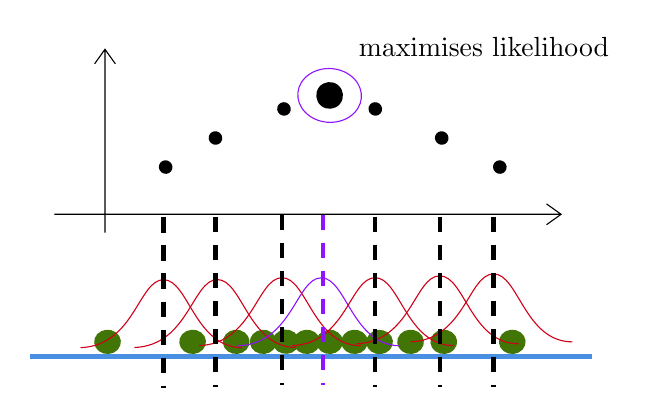
\begin{tikzpicture}[x=0.75pt,y=0.75pt,yscale=-1,xscale=1]
%uncomment if require: \path (0,195.33333206176758); %set diagram left start at 0, and has height of 195.33333206176758

%Flowchart: Connector [id:dp16864482457380792] 
\draw  [draw opacity=0][fill={rgb, 255:red, 65; green, 117; blue, 5 }  ,fill opacity=1 ] (75.71,159.09) .. controls (72.96,157.04) and (68.9,157.42) .. (66.65,159.93) .. controls (64.4,162.44) and (64.81,166.13) .. (67.57,168.17) .. controls (70.33,170.21) and (74.39,169.84) .. (76.63,167.33) .. controls (78.88,164.82) and (78.47,161.13) .. (75.71,159.09) -- cycle ;
%Flowchart: Connector [id:dp9802591055616827] 
\draw  [draw opacity=0][fill={rgb, 255:red, 65; green, 117; blue, 5 }  ,fill opacity=1 ] (137.71,159.09) .. controls (134.96,157.04) and (130.9,157.42) .. (128.65,159.93) .. controls (126.4,162.44) and (126.81,166.13) .. (129.57,168.17) .. controls (132.33,170.21) and (136.39,169.84) .. (138.63,167.33) .. controls (140.88,164.82) and (140.47,161.13) .. (137.71,159.09) -- cycle ;
%Flowchart: Connector [id:dp05225203779633203] 
\draw  [draw opacity=0][fill={rgb, 255:red, 65; green, 117; blue, 5 }  ,fill opacity=1 ] (116.71,159.09) .. controls (113.96,157.04) and (109.9,157.42) .. (107.65,159.93) .. controls (105.4,162.44) and (105.81,166.13) .. (108.57,168.17) .. controls (111.33,170.21) and (115.39,169.84) .. (117.63,167.33) .. controls (119.88,164.82) and (119.47,161.13) .. (116.71,159.09) -- cycle ;
%Flowchart: Connector [id:dp2760284772295425] 
\draw  [draw opacity=0][fill={rgb, 255:red, 65; green, 117; blue, 5 }  ,fill opacity=1 ] (171.71,159.09) .. controls (168.96,157.04) and (164.9,157.42) .. (162.65,159.93) .. controls (160.4,162.44) and (160.81,166.13) .. (163.57,168.17) .. controls (166.33,170.21) and (170.39,169.84) .. (172.63,167.33) .. controls (174.88,164.82) and (174.47,161.13) .. (171.71,159.09) -- cycle ;
%Flowchart: Connector [id:dp6624437432554011] 
\draw  [draw opacity=0][fill={rgb, 255:red, 65; green, 117; blue, 5 }  ,fill opacity=1 ] (150.71,159.09) .. controls (147.96,157.04) and (143.9,157.42) .. (141.65,159.93) .. controls (139.4,162.44) and (139.81,166.13) .. (142.57,168.17) .. controls (145.33,170.21) and (149.39,169.84) .. (151.63,167.33) .. controls (153.88,164.82) and (153.47,161.13) .. (150.71,159.09) -- cycle ;
%Flowchart: Connector [id:dp03313254158829326] 
\draw  [draw opacity=0][fill={rgb, 255:red, 65; green, 117; blue, 5 }  ,fill opacity=1 ] (194.71,159.09) .. controls (191.96,157.04) and (187.9,157.42) .. (185.65,159.93) .. controls (183.4,162.44) and (183.81,166.13) .. (186.57,168.17) .. controls (189.33,170.21) and (193.39,169.84) .. (195.63,167.33) .. controls (197.88,164.82) and (197.47,161.13) .. (194.71,159.09) -- cycle ;
%Flowchart: Connector [id:dp8229616225061853] 
\draw  [draw opacity=0][fill={rgb, 255:red, 65; green, 117; blue, 5 }  ,fill opacity=1 ] (182.71,159.09) .. controls (179.96,157.04) and (175.9,157.42) .. (173.65,159.93) .. controls (171.4,162.44) and (171.81,166.13) .. (174.57,168.17) .. controls (177.33,170.21) and (181.39,169.84) .. (183.63,167.33) .. controls (185.88,164.82) and (185.47,161.13) .. (182.71,159.09) -- cycle ;
%Flowchart: Connector [id:dp7001184718325861] 
\draw  [draw opacity=0][fill={rgb, 255:red, 65; green, 117; blue, 5 }  ,fill opacity=1 ] (221.71,159.09) .. controls (218.96,157.04) and (214.9,157.42) .. (212.65,159.93) .. controls (210.4,162.44) and (210.81,166.13) .. (213.57,168.17) .. controls (216.33,170.21) and (220.39,169.84) .. (222.63,167.33) .. controls (224.88,164.82) and (224.47,161.13) .. (221.71,159.09) -- cycle ;
%Flowchart: Connector [id:dp48826326309342183] 
\draw  [draw opacity=0][fill={rgb, 255:red, 65; green, 117; blue, 5 }  ,fill opacity=1 ] (206.78,159.16) .. controls (204.02,157.12) and (199.96,157.49) .. (197.71,160) .. controls (195.46,162.51) and (195.88,166.2) .. (198.63,168.24) .. controls (201.39,170.28) and (205.45,169.91) .. (207.7,167.4) .. controls (209.94,164.89) and (209.53,161.2) .. (206.78,159.16) -- cycle ;
%Flowchart: Connector [id:dp7605140271867799] 
\draw  [draw opacity=0][fill={rgb, 255:red, 65; green, 117; blue, 5 }  ,fill opacity=1 ] (270.71,159.09) .. controls (267.96,157.04) and (263.9,157.42) .. (261.65,159.93) .. controls (259.4,162.44) and (259.81,166.13) .. (262.57,168.17) .. controls (265.33,170.21) and (269.39,169.84) .. (271.63,167.33) .. controls (273.88,164.82) and (273.47,161.13) .. (270.71,159.09) -- cycle ;
%Flowchart: Connector [id:dp9918467121427432] 
\draw  [draw opacity=0][fill={rgb, 255:red, 65; green, 117; blue, 5 }  ,fill opacity=1 ] (237.71,159.09) .. controls (234.96,157.04) and (230.9,157.42) .. (228.65,159.93) .. controls (226.4,162.44) and (226.81,166.13) .. (229.57,168.17) .. controls (232.33,170.21) and (236.39,169.84) .. (238.63,167.33) .. controls (240.88,164.82) and (240.47,161.13) .. (237.71,159.09) -- cycle ;
%Flowchart: Connector [id:dp6215197594198278] 
\draw  [draw opacity=0][fill={rgb, 255:red, 65; green, 117; blue, 5 }  ,fill opacity=1 ] (161.65,159.02) .. controls (158.89,156.97) and (154.84,157.35) .. (152.59,159.86) .. controls (150.34,162.36) and (150.75,166.05) .. (153.51,168.1) .. controls (156.27,170.14) and (160.32,169.77) .. (162.57,167.26) .. controls (164.82,164.75) and (164.41,161.06) .. (161.65,159.02) -- cycle ;
%Curve Lines [id:da2652484332595779] 
\draw [color={rgb, 255:red, 208; green, 2; blue, 27 }  ,draw opacity=1 ]   (58.63,166.42) .. controls (84.63,165.51) and (86.63,133.68) .. (98.63,133.68) .. controls (110.63,133.68) and (113.63,166.42) .. (136.63,166.42) ;


%Curve Lines [id:da514115735600639] 
\draw [color={rgb, 255:red, 208; green, 2; blue, 27 }  ,draw opacity=1 ]   (84.57,166.35) .. controls (110.57,165.44) and (112.57,133.61) .. (124.57,133.61) .. controls (136.57,133.61) and (139.57,166.35) .. (162.57,166.35) ;


%Curve Lines [id:da48620018179231006] 
\draw [color={rgb, 255:red, 208; green, 2; blue, 27 }  ,draw opacity=1 ]   (115.71,165.46) .. controls (141.71,164.55) and (143.71,132.72) .. (155.71,132.72) .. controls (167.71,132.72) and (170.71,165.46) .. (193.71,165.46) ;


%Curve Lines [id:da5475113930938333] 
\draw [color={rgb, 255:red, 144; green, 19; blue, 254 }  ,draw opacity=1 ]   (134.63,165.51) .. controls (160.63,164.6) and (162.63,132.77) .. (174.63,132.77) .. controls (186.63,132.77) and (189.63,165.51) .. (212.63,165.51) ;


%Curve Lines [id:da6603466688287307] 
\draw [color={rgb, 255:red, 208; green, 2; blue, 27 }  ,draw opacity=1 ]   (160.57,165.44) .. controls (186.57,164.53) and (188.57,132.7) .. (200.57,132.7) .. controls (212.57,132.7) and (215.57,165.44) .. (238.57,165.44) ;


%Curve Lines [id:da7350885388643735] 
\draw [color={rgb, 255:red, 208; green, 2; blue, 27 }  ,draw opacity=1 ]   (191.71,164.55) .. controls (217.71,163.64) and (219.71,131.81) .. (231.71,131.81) .. controls (243.71,131.81) and (246.71,164.55) .. (269.71,164.55) ;


%Curve Lines [id:da8167876559532401] 
\draw [color={rgb, 255:red, 208; green, 2; blue, 27 }  ,draw opacity=1 ]   (217.64,163.63) .. controls (243.64,162.72) and (245.64,130.89) .. (257.64,130.89) .. controls (269.64,130.89) and (272.64,163.63) .. (295.64,163.63) ;


%Shape: Axis 2D [id:dp13149341674890747] 
\draw  (46,102.17) -- (290.17,102.17)(70.42,22.67) -- (70.42,111) (283.17,97.17) -- (290.17,102.17) -- (283.17,107.17) (65.42,29.67) -- (70.42,22.67) -- (75.42,29.67)  ;
%Straight Lines [id:da6554257366346852] 
\draw [color={rgb, 255:red, 74; green, 144; blue, 226 }  ,draw opacity=1 ][line width=1.5]    (34.17,170.67) -- (305.17,170.67) ;


%Straight Lines [id:da04519936834215055] 
\draw [color={rgb, 255:red, 0; green, 0; blue, 0 }  ,draw opacity=1 ][line width=1.5]  [dash pattern={on 5.63pt off 4.5pt}]  (98.63,103.67) -- (98.63,185.67) ;


%Straight Lines [id:da0546936538883096] 
\draw [color={rgb, 255:red, 0; green, 0; blue, 0 }  ,draw opacity=1 ][line width=1.5]  [dash pattern={on 5.63pt off 4.5pt}]  (123.63,103.33) -- (123.63,185.33) ;


%Straight Lines [id:da034029900096602006] 
\draw [color={rgb, 255:red, 0; green, 0; blue, 0 }  ,draw opacity=1 ][line width=1.5]  [dash pattern={on 5.63pt off 4.5pt}]  (155.63,102.33) -- (155.63,184.33) ;


%Straight Lines [id:da7302167475214083] 
\draw [color={rgb, 255:red, 0; green, 0; blue, 0 }  ,draw opacity=1 ][line width=1.5]  [dash pattern={on 5.63pt off 4.5pt}]  (200.63,103.33) -- (200.63,185.33) ;


%Straight Lines [id:da7572917651815845] 
\draw [color={rgb, 255:red, 0; green, 0; blue, 0 }  ,draw opacity=1 ][line width=1.5]  [dash pattern={on 5.63pt off 4.5pt}]  (231.63,103.33) -- (231.63,185.33) ;


%Straight Lines [id:da1834654835330778] 
\draw [color={rgb, 255:red, 0; green, 0; blue, 0 }  ,draw opacity=1 ][line width=1.5]  [dash pattern={on 5.63pt off 4.5pt}]  (257.63,103.33) -- (257.63,185.33) ;


%Straight Lines [id:da32238508942428457] 
\draw [color={rgb, 255:red, 144; green, 19; blue, 254 }  ,draw opacity=1 ][line width=1.5]  [dash pattern={on 5.63pt off 4.5pt}]  (175.63,102.33) -- (175.63,184.33) ;


%Flowchart: Connector [id:dp9444134217748508] 
\draw  [draw opacity=0][fill={rgb, 255:red, 0; green, 0; blue, 0 }  ,fill opacity=1 ] (182.71,39.91) .. controls (179.96,37.66) and (175.9,38.07) .. (173.65,40.83) .. controls (171.4,43.59) and (171.81,47.64) .. (174.57,49.89) .. controls (177.33,52.14) and (181.39,51.73) .. (183.63,48.97) .. controls (185.88,46.21) and (185.47,42.16) .. (182.71,39.91) -- cycle ;
%Flowchart: Connector [id:dp7514426273907349] 
\draw  [draw opacity=0][fill={rgb, 255:red, 0; green, 0; blue, 0 }  ,fill opacity=1 ] (158.69,48.91) .. controls (157.27,47.76) and (155.21,47.94) .. (154.09,49.32) .. controls (152.96,50.71) and (153.19,52.76) .. (154.61,53.91) .. controls (156.02,55.07) and (158.08,54.88) .. (159.21,53.5) .. controls (160.33,52.12) and (160.1,50.06) .. (158.69,48.91) -- cycle ;
%Flowchart: Connector [id:dp3682543414210395] 
\draw  [draw opacity=0][fill={rgb, 255:red, 0; green, 0; blue, 0 }  ,fill opacity=1 ] (202.69,48.91) .. controls (201.27,47.76) and (199.21,47.94) .. (198.09,49.32) .. controls (196.96,50.71) and (197.19,52.76) .. (198.61,53.91) .. controls (200.02,55.07) and (202.08,54.88) .. (203.21,53.5) .. controls (204.33,52.12) and (204.1,50.06) .. (202.69,48.91) -- cycle ;
%Flowchart: Connector [id:dp24505487020864902] 
\draw  [draw opacity=0][fill={rgb, 255:red, 0; green, 0; blue, 0 }  ,fill opacity=1 ] (234.69,62.91) .. controls (233.27,61.76) and (231.21,61.94) .. (230.09,63.32) .. controls (228.96,64.71) and (229.19,66.76) .. (230.61,67.91) .. controls (232.02,69.07) and (234.08,68.88) .. (235.21,67.5) .. controls (236.33,66.12) and (236.1,64.06) .. (234.69,62.91) -- cycle ;
%Flowchart: Connector [id:dp790226000694918] 
\draw  [draw opacity=0][fill={rgb, 255:red, 0; green, 0; blue, 0 }  ,fill opacity=1 ] (262.69,76.91) .. controls (261.27,75.76) and (259.21,75.94) .. (258.09,77.32) .. controls (256.96,78.71) and (257.19,80.76) .. (258.61,81.91) .. controls (260.02,83.07) and (262.08,82.88) .. (263.21,81.5) .. controls (264.33,80.12) and (264.1,78.06) .. (262.69,76.91) -- cycle ;
%Flowchart: Connector [id:dp6717973952893042] 
\draw  [draw opacity=0][fill={rgb, 255:red, 0; green, 0; blue, 0 }  ,fill opacity=1 ] (125.69,62.91) .. controls (124.27,61.76) and (122.21,61.94) .. (121.09,63.32) .. controls (119.96,64.71) and (120.19,66.76) .. (121.61,67.91) .. controls (123.02,69.07) and (125.08,68.88) .. (126.21,67.5) .. controls (127.33,66.12) and (127.1,64.06) .. (125.69,62.91) -- cycle ;
%Flowchart: Connector [id:dp7185747228456638] 
\draw  [draw opacity=0][fill={rgb, 255:red, 0; green, 0; blue, 0 }  ,fill opacity=1 ] (101.69,76.91) .. controls (100.27,75.76) and (98.21,75.94) .. (97.09,77.32) .. controls (95.96,78.71) and (96.19,80.76) .. (97.61,81.91) .. controls (99.02,83.07) and (101.08,82.88) .. (102.21,81.5) .. controls (103.33,80.12) and (103.1,78.06) .. (101.69,76.91) -- cycle ;
%Flowchart: Connector [id:dp6253213348265279] 
\draw  [color={rgb, 255:red, 144; green, 19; blue, 254 }  ,draw opacity=1 ] (188.19,34.94) .. controls (181.57,30.36) and (171.93,31.09) .. (166.65,36.59) .. controls (161.38,42.09) and (162.47,50.27) .. (169.09,54.86) .. controls (175.71,59.44) and (185.36,58.71) .. (190.63,53.21) .. controls (195.9,47.71) and (194.81,39.53) .. (188.19,34.94) -- cycle ;

% Text Node
\draw (253,21.33) node   [align=left] {maximises likelihood};


\end{tikzpicture}
\end{YTB_SUMM}

\newpage

\chapter[Time Series Models]{Time Series Models (12.5\% à 17.5\%)}

\subsection{Information}

\begin{distributions}[Objective]
Understand key concepts concerning regression-based time series models.
\end{distributions}

\begin{outcomes}[Learning outcomes]
\begin{enumerate}
	\item	Définir et expliquer les concepts, et composantes, des processus de séries chronologiques stochastiques. Incluant:
	\begin{itemize}
		\item	Les marches aléatoires
		\item	Stationnarité
		\item	Auto-corrélation
	\end{itemize}
	\item	Décrire des modèles de séries chronologiques précis dont:
	\begin{itemize}
		\item	Exponential smoothing
		\item	Autoregressive
		\item	Autoregressive conditionally heteroskedastic models
	\end{itemize}
	\item	Calculer et interpréter les valeurs prédites et leurs intervalles de confiance.
\end{enumerate}
\end{outcomes}

\begin{ASM_chapter}[Related lessons ASM]
\begin{enumerate}
  \setcounter{enumi}{18}
	\item	Time Series: Basics
	\item	Time Series: Autoregressive Models
	\item	Time Series: Forecasting Models
\end{enumerate}
\end{ASM_chapter}

\begin{YTB_vids}[Vidéos YouTube]
\begin{itemize}
	\item	\href{https://www.youtube.com/watch?v=-gmlyRRscXo}{Ben Lambert: Time series vs cross sectional data}
	\item	\href{https://www.youtube.com/watch?v=bWo_ka37szw&list=PLvo9ZnEQG5oXC-cg8ecXr6SJZWprEL1UC&index=3}{Ben Lambert: Time series Gauss Markov conditions}
	\item	\href{https://www.youtube.com/watch?v=DeORzP0go5I&list=PLvcbYUQ5t0UHOLnBzl46_Q6QKtFgfMGc3&index=14}{ritvikmath: Time Series Talk : Autocorrelation and Partial Autocorrelation}
	\item	\href{https://www.youtube.com/watch?v=oY-j2Wof51c&list=PLvcbYUQ5t0UHOLnBzl46_Q6QKtFgfMGc3&index=6}{ritvikmath: Time Series Talk: Stationarity}
	\item	\href{https://www.youtube.com/watch?v=cr4zIXAmSRI}{ritvikmath: Time Series Talk : White Noise}
%	\item	\href{https://www.youtube.com/watch?v=VPNijQ2L3XM&list=PLvcbYUQ5t0UHOLnBzl46_Q6QKtFgfMGc3&index=4}{ritvikmath: Time Series Talk : Lag operator}
	\item	\href{https://www.youtube.com/watch?v=5-2C4eO4cPQ}{ritvikmath: Time Series Talk : Autoregressive Model}
%	\item	\href{https://www.youtube.com/watch?v=voryLhxiPzE&list=PLvcbYUQ5t0UHOLnBzl46_Q6QKtFgfMGc3&index=11}{ritvikmath: Time Series Talk: Moving Average}
%	\item	\href{https://www.youtube.com/watch?v=_tgB-ri9-8c&list=PLvcbYUQ5t0UHOLnBzl46_Q6QKtFgfMGc3&index=10}{ritvikmath: Time Series Talk: Moving Average and ACF}
%	\item	\href{https://www.youtube.com/watch?v=HhvTlaN06AM&list=PLvcbYUQ5t0UHOLnBzl46_Q6QKtFgfMGc3&index=9}{ritvikmath: Time Series Talk: ARMA Model}
%	\item	\href{https://www.youtube.com/watch?v=Li95a2biFCU&list=PLvcbYUQ5t0UHOLnBzl46_Q6QKtFgfMGc3&index=8}{ritvikmath: Time Series Talk: ARCH Model}
%	\item	\href{https://www.youtube.com/watch?v=3UmyHed0iYE&list=PLvcbYUQ5t0UHOLnBzl46_Q6QKtFgfMGc3&index=5}{ritvikmath: Time Series Talk: ARIMA Model}
%	\item	\href{https://www.youtube.com/watch?v=4hrMdu9CSQs&list=PLvcbYUQ5t0UHOLnBzl46_Q6QKtFgfMGc3&index=3}{ritvikmath: Time Series Talk: What is seasonality?}
%	\item	\href{https://www.youtube.com/watch?v=WjeGUs6mzXg&list=PLvcbYUQ5t0UHOLnBzl46_Q6QKtFgfMGc3&index=2}{ritvikmath: Time Series Talk: Seasonal ARIMA Model}
\end{itemize}
\end{YTB_vids}

\subsection{Résumés des chapitres}

\begin{CHPT_SUMM}{19. Time Series: Basics}
Time series -> Séries chronologiques
\begin{enumerate}
	\item	\textbf{Introduction}
	\begin{itemize}
		\item	\textbf{Séries chronologiques}: Série d'observations $y_{1}, y_{2}, \dots, y_{T}$ sur des intervalles de temps consécutives;
		\item	\textbf{Analyse de séries chronologiques}: Essayer de déchiffrer des patterns dans les séries chrono pour en faire des prévisions;
		\item[]	Ces patterns peuvent prendre plusieurs formes y inclut de relier les observations $y_{t}$ aux observations précédentes de la série ou, au temps lui-même;
		\item	\textbf{Données longitudinales}: Données d'un processus variant avec le temps;
		\item	Des données \textbf{cross-sectional} sont l'inverse, elles ne sont pas organisées chronologiquement;
		\item	Un \textbf{causal model} est un modèle sans variables explicatives reliées au temps;
		\item[]	Caveat: Les modèles statistiques dépistent la corrélation et non la causalité;
		\item[]	En revanche, des modèles de séries chronologiques peuvent trouver des relations causales avec le temps;
		\item[]	Caveat: Des modèles statistiques doivent connaître les valeurs des variables indépendantes pour faire des prévisions de la variable dépendante;
		\item	3 composantes aux séries chronologiques:
		\begin{enumerate}
			\item	\textbf{Trend} $T_{t}$: Long term pattern des données;
			\item	\textbf{Seasonality} $S_{t}$: Cyclical pattern des données;
			\item	\textbf{Random patterns};
		\end{enumerate}	
		\item	On utilise un scatter plot du modèle et du temps, i.e. un \textbf{time series plot}, afin de évaluer la série chronologique;
		\item[]	\textbf{Seasonal adjustment} Pour prendre en compte les seasonal patterns on peut ajuster le modèle avec une variable binaire;
		\item	\textbf{Regime change}: Pour prendre en compte un behaviour change on peut ajuster le modèle avec une variable binaire débutant à un point fixé dans le temps;
		\item	Les modèles de séries chronologiques adressent quelques problèmes des modèles de régression:		
		\begin{itemize}
			\item	Les modèles de régression sont \textbf{naïve dans le sens qu'ils ignorent l'information autre que la série chronologique étant ajusté}.
			\item	\textit{Un autre négatif est que le modèle de régression allouent plus de poids aux observations récentes (celles ayant les statistiques $t$ les plus éloignés de la moyenne)};
			\item	La différence en modélisation de données chronologiques vs transversales est bien expliquée dans le vidéo de Ben Lambert;
		\end{itemize} 
	\end{itemize}
	\item	\textbf{Mean} and \textbf{variance}
	\begin{itemize}
		\item	Si la \textbf{moyenne} \textit{(au temps t)} $\text{E}[y_{t}] = \mu(t)$ ne varie pas dans le temps, la série est dite d'avoir une espérance \textbf{stationnaire};
		\item	Ce faisant, on peut l'estimer avec les valeurs observées;
		\item	Pareillement, si la \textbf{variance} \textit{(au temps t)} $\text{Var}(y_{t}) = \sigma^{2}(t)$ ne varie pas dans le temps, la série est dite d'avoir une variance \textbf{stationnaire} et on peut l'estimer avec la variance échantillonnale;
		\item[]	Sinon, $\sigma^{2}(t) = \text{E}[(y_{t} - \mu(t))^{2}]$;
		\begin{itemize}
			\item	On s'attend à de la corrélation. Ceci implique que la variance échantillonnale va sous-estimer la vraie variance;
			\item	Cependant, le biais décroît rapidement lorsque la taille de la série augmente;
		\end{itemize}
		\item	\textbf{Autocorrelation} ou \textit{serial correlation}: voir formule pour l'auto-corrélation échantillonnale $r_{k}$.
		\begin{itemize}
			\item	Le distance $k$ des observations d'une série chronologique au temps $t$ avec la même série au temps $t + k$ est le \textbf{lag};
			\item	Si la série à une espérance stationnaire, et que la variance et corrélation sont fonction seulement du \textit{lag} et non du temps lui-même, la série est dite \textbf{\textit{(weakly)} stationary} \textbf{(par défaut)};
			\item	Si aucun des moments plus élevés varient avec le temps, alors la série est \textbf{\textit{strongly} stationary};
		\end{itemize}
	\end{itemize}
	\item	\textbf{White noise}: Une série chronologique \textbf{white noise} est caractérisé par:
	\begin{itemize}
		\item	L'indépendance des termes;
		\item[]	Ce faisant, la corrélation $r_{k}$ à tous \textbf{lag} supérieurs à 0 est de 0 ($r_{0}$ est toujours égale à 1);
		\item	Une espérance constante $\mu$;
		\item	Une variance constante $\sigma^{2}$;
		\item	Habituellement, on suppose la normalité;
	\end{itemize}
	\item[]	Réduction de série, alias \textbf{time series \textit{filtering}}:
	\begin{itemize}
		\item	Nous voulons toujours réduire toute série chronologique à une série white noise en identifiant des patterns;
		\item	La partie inexplicable par les patterns qui demeurent est dite d'être \textbf{irréductible} et est donc traitée comme du \textbf{\textit{white noise}};
		\item	On peut donc penser à ceci comme l'équivalent de l'erreur $\varepsilon$ en régression pour les séries chronologiques;
		\item	Pour des \hyperref[sec:ex_rand_walk]{exemples}, voir la fin de la section de marches aléatoires;
	\end{itemize}
	 et en laissant l'imprévisible comme du white noise
	\item	\textbf{Marches aléatoires}: Une \textbf{marche aléatoire} est:
	\begin{itemize}
		\item	Une série chronologique \textbf{\textit{non}-stationnaire};
		\item	Ayant comme valeur le niveau initial $y_{0}$ plus l'accumulation du \textit{white noise} $c_{t}$;
		\item	L'expression est donc de forme: $y_{t} = y_{t - 1} + c_{t}, t \ge 1$.
	\end{itemize}
	\item[]	Voir les formules des espérances / variances;
	\begin{itemize}
		\item	Habituellement, $\text{E}[c_{t}] = \mu_{c} = 0$ mais l'auteur le défini plus généralement;
		\item	Si $\mu_{c} = 0$ la série est néanmoins non-stationnaire puisque la variance croît avec le temps;
		\item	Si $\mu_{c} \neq 0$ la série est une marche aléatoire \textbf{avec drift} où $\mu_{c}$ est le drift;
		\item	On déduit de plus que la différence entre marches aléatoires $y_{t} - y_{t - 1}$ est du white noise;
	\end{itemize}
	\item[]	Pour distinguer et comprendre la distinction entre une tendance dans le temps (à gauche) et une marche aléatoire (à droite) on compare les deux:
	\begin{align*}
		y_{t}	&= 	y_{0} + t k + \varepsilon_{t}	&
		&\text{vs}	&
		y_{t}	&= 	y_{0} + t \mu_{c}  + \sum_{j = 1}^{t} \varepsilon_{j}	
	\end{align*}
	D'où le lien entre l'erreur et le white noise s'éclaircit. Malgré une espérance identique si $k = \mu_{c}$, la variance de la série chrono va croître avec le temps;
	\item[]	\label{sec:ex_rand_walk} Exemples de \textbf{filtering}: 
	\begin{itemize}
		\item	Différencier une marche aléatoire;
		\item	Prendre le log de la série. Ceci peut stabiliser la variance;
		\item	Finalement, prendre le log de la différence des séries qui correspond \textit{approximativement} à des changements proportionnels;
	\end{itemize}
	\item	\textbf{Control charts}: Graphique pour observer l'évolution d'un processus avec le temps.
	\begin{itemize}
		\item	Les données sont placées en ordre chronologique;
		\item	Le graphique comporte une ligne centrale pour la moyenne et deux lignes pour les bornes supérieures et inférieures (typiquement Q1 et Q3);
		\item	L'axe des y sert à évaluer la moyenne du processus et l'axe des x permet d'observer l'étendu;
		\item	Ce faisant, l'utilité est un peu semblable à celle d'un boxplot. On évalue si un processus est relativement stable en observant leur distribution relative au temps. En revanche, un boxplot permet vérifier que les données n'ont pas trop de points abérrants et qu’elles ne sont pas trop répandues.;
		\item	On peut donc évaluer si un processus est stable (en contrôle) ou instable (hors de contrôle)
	\end{itemize}
	\item[]	\textbf{Xbar charts}: Calculer la moyenne des séries de $k$ observations.
		\begin{itemize}
		\item	Par exemple avec $k = 5$, on calcule la moyenne des observations 1 à 5, 6 à 10, 11 à 15, etc.;
		\item	Puisque la variance des moyennes sera plus faible que la variance de la série, des tendances inhabituelles devraient être plus apparentes;
		\end{itemize}
	\item[]	\textbf{R charts}: Calculer l'étendu des séries de $k$ observations.
		\begin{itemize}
		\item	L'étendu est la valeur maximale - la valeur minimale;
		\item	Ceci donne une idée de la dispersion des données pour évaluer la volatilité et évaluer des patterns;
		\end{itemize}
	\item	\textbf{Evaluating forecasts} \textit{(évaluer les prévisions)}
	\item[]	On utilise le \textbf{out-of-sample validation}
		\begin{itemize}
		\item	Les données sont partitionnées jusqu'au point fixe $T_{1}$ où $T_{1} < T$;
		\item	Ces données sont utilisés pour ajuster le modèle et le reste pour le tester;
		\item	Avec les données de test on calcule le résidu $e_{t} = \hat{y}_{t} - y_{t}$;
		\end{itemize}
	\item[]	Par la suite on évalue la qualité du modèle avec ces statistiques \emph{(voir formules)}:
	\begin{itemize}
		\item	Le \textbf{Mean Error} (ME) et \textbf{Mean Percentage Error} (MPE) détectent des \textbf{trend patterns};
		\item	\textbf{Cependant}, ils ne \textbf{détectent pas} des problèmes lorsque les \textit{résidus sont positifs et négatifs} avec une \textit{moyenne faible} alors que les \textbf{autres mesures oui};
		\item	De plus, MPE ne peut pas être utilisé lorsque la série contient des 0s et peut être incohérente avec des termes négatifs;
		\item	Le \textbf{Mean Square Error} (MSE) et \textbf{Mean Absolute Error} (MAE) adressent le problème de résidus nuls avec ME et le \textbf{Mean Absolute Percentage Error} (MAPE) pour le MPE;
		\item	Cependant, le MAPE a les même problèmes que le MPE avec les termes nuls;
	\end{itemize}
\end{enumerate}
\textbf{Note sur les exercices:} 
\begin{enumerate}
	\item	
\end{enumerate}
\end{CHPT_SUMM}

\begin{FORMULA_SUMM}{Formules chapitre 19}
\textbf{ASTUCE}: La corrélation échantillonnale peut être calculé avec la TI-30XS. $r_{k} = \frac{\sum X^{2}}{\sum XY}$ où la colonne des $X$ exclue le  premier terme et la colonne des $Y$ le dernier.
\begin{align*}
	s^{2}	&=	\frac{\sum_{t = 1}^{n}(y_{t} - \bar{y})^{2}}{n - 1}	&
	r_{k}	&=	\frac{\sum_{t = k + 1}^{T}(y_{t - k} - \bar{y})(y_{t} - \bar{y})}{\sum_{t = 1}^{T}(y_{t} - \bar{y})^{2}}	\\
	r_{0}	&=	1
\end{align*}
\begin{align*}
	ME	&=	\frac{1}{T - T_{1}} \sum_{t = T_{1}}^{T} e_{t}	&
	MPE	&=	\frac{100}{T - T_{1}} \sum_{t = T_{1}}^{T} \frac{e_{t}}{y_{t}}	\\
	MSE	&=	\frac{1}{T - T_{1}} \sum_{t = T_{1}} e_{t}^{2}	\\
	MAE	&=	\frac{1}{T - T_{1}} \sum_{t = T_{1}}^{T} |e_{t}|	&	
	MAPE	&=	\frac{100}{T - T_{1}} \sum_{t = T_{1}}^{T} \left| \frac{e_{t}}{y_{t}}\right|	\\
\end{align*}
Pour une marche aléatoire $y_{t}$ avec la série white noise $c_{t}$:
\begin{align*}
	y_{t}	&= 	y_{t - 1} + c_{t},	t \ge 1	\\
	\text{E}[c_{t}]	&=	\mu_{c}	&
	\text{Var}(c_{t})	&=	\sigma^{2}_{c}	\\
	\text{E}[y_{t}]	&=	y_{0} + t \mu_{c}	&
	\text{Var}(y_{t})	&=	t \sigma^{2}_{c}	\\	
	y_{T + l}	&= 	y_{T} + l \bar{c}	
\end{align*}
$\bar{c}$ est la moyenne échantillonnale de $c_{t}$.

\begin{tabular}{|l|l|l|}
\hline
\rowcolor[HTML]{21650A} 
		\multicolumn{1}{|c|}{\cellcolor[HTML]{21650A}{\color[HTML]{FFFFFF} \textbf{Measure}}}                
	&	\multicolumn{1}{c|}{\cellcolor[HTML]{21650A}{\color[HTML]{FFFFFF} \textbf{White noise}}}	
	&	\multicolumn{1}{c|}{\cellcolor[HTML]{21650A}{\color[HTML]{FFFFFF} \textbf{Random walk}}}	\\	
\hline
\rowcolor[HTML]{B8F0A5}	$l$-period lookahead forecast &	$\hat{y}_{T + l} = \bar{y} \; \forall l$	&	$\hat{y}_{T + l} = y_{T} + l \bar{c}$	\\	
\hline
%\rowcolor[HTML]{B8F0A5}	Forecast interval of $y_{T + l}$	&	$\bar{y} \pm t_{T - 1, 1 - \frac{\alpha}{2}} s_{y}\sqrt{1 + \frac{1}{T}}$	&	de niveau \\	\hline
\rowcolor[HTML]{B8F0A5}	Estimated standard error $se_{\hat{y}_{T + l}}$	&	$s_{y}\sqrt{1 + \frac{1}{T}}$	&	$s_{w}\sqrt{l}$ 	\\ \hline
\end{tabular}
où $w_{t} = y_{t} - y_{t - 1}$.

\end{FORMULA_SUMM}

\begin{CHPT_SUMM}{20. Time Series: Autoregressive Models}
\textbf{Pas encore fait, notes pour me donner une idée du chapitre}
\begin{enumerate}
	\item	Intro
	\begin{itemize}
		\item	AR(1) model is a time series where each term may be expressed in terms of the previous term plus white noise;
		\item	Examples;
		\item	Stationnarity;
		\item	True autocorrelation at lag $k$;
		\item	Coefficients;
	\end{itemize}
	\item	Forecasting with AR(1) series
\end{enumerate}
\textbf{Note sur les exercices:} 
\begin{enumerate}
	\item	
\end{enumerate}
\end{CHPT_SUMM}

\begin{CHPT_SUMM}{21. Time Series: Forecasting Models}
\textbf{Pas encore fait, notes pour me donner une idée du chapitre}
\begin{enumerate}
	\item	Moving average smoothing
	\begin{itemize}
		\item	Average $k$ consecutive terms and create a new time series
		\item	Moving average smoothing is weighted least square with weights of 1 on the most recent $k$ periods and 0 on earlier periods;
	\end{itemize}
	\item	Exponential smoothing
	\begin{itemize}
		\item	Moving average weights are constant for the $k$ previous periods and then drop off to 0;
		\item	To have a smoother pattern of weights, use exponential smoothing to put weights that're proportionnal;
		\item	Impact of different weights;
	\end{itemize}
	\item	Seasonal models
	\begin{itemize}
		\item	Fixed effects;
		\item	Autoregressive seasonal models;
		\item	Seasonal exponential smoothing;
	\end{itemize}
	\item	Unit root tests
	\item	ARCH and GARCH models
\end{enumerate}
\textbf{Note sur les exercices:} 
\begin{enumerate}
	\item	
\end{enumerate}
\end{CHPT_SUMM}

\subsection{Notes sur les vidéos YouTube}

\begin{YTB_SUMM}{\href{https://www.youtube.com/watch?v=-gmlyRRscXo}{Ben Lambert: Time series vs cross sectional data}}
Le vidéo est utile pour commencer à conceptualiser la différence en approche des données auxquelles nous sommes habituées (\textit{cross-sectional data}) des données de séries chronologiques.

Pour ce, et les prochains vidéos de Ben Lambert, $u_{t} = \varepsilon_{t}$.

\begin{minipage}{0.2\linewidth}
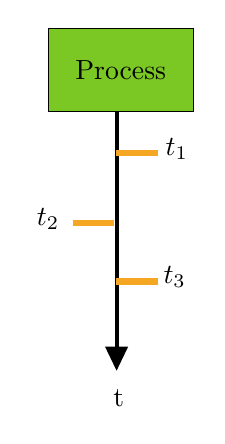
\begin{tikzpicture}[x=0.75pt,y=0.75pt,yscale=-1,xscale=1]
%uncomment if require: \path (0,300); %set diagram left start at 0, and has height of 300

%Shape: Rectangle [id:dp45341716963014833] 
\draw  [fill={rgb, 255:red, 109; green, 194; blue, 12 }  ,fill opacity=0.9 ] (74,51) -- (144,51) -- (144,91) -- (74,91) -- cycle ;
%Straight Lines [id:da3471781120754416] 
\draw [line width=1.5]    (107,91) -- (107,212) ;
\draw [shift={(107,216)}, rotate = 270] [fill={rgb, 255:red, 0; green, 0; blue, 0 }  ][line width=0.08]  [draw opacity=0] (11.61,-5.58) -- (0,0) -- (11.61,5.58) -- cycle    ;

%Straight Lines [id:da24464797721586562] 
\draw [color={rgb, 255:red, 245; green, 166; blue, 35 }  ,draw opacity=1 ][line width=2.25]    (85.83,145) -- (105.83,145) ;

%Straight Lines [id:da022853384994410142] 
\draw [color={rgb, 255:red, 245; green, 166; blue, 35 }  ,draw opacity=1 ][line width=2.25]    (106.83,173) -- (126.83,173) ;

%Straight Lines [id:da31936638200020173] 
\draw [color={rgb, 255:red, 245; green, 166; blue, 35 }  ,draw opacity=1 ][line width=2.25]    (106.83,111) -- (126.83,111) ;

% Text Node
\draw (108,229) node   [align=left] {t};
% Text Node
\draw (136,109) node   [align=left] {$\displaystyle t_{1}$};
% Text Node
\draw (74,143) node   [align=left] {$\displaystyle t_{2}$};
% Text Node
\draw (135,171) node   [align=left] {$\displaystyle t_{3}$};
% Text Node
\draw (109,71) node   [align=left] {Process};
\end{tikzpicture}
\end{minipage}
\begin{minipage}{0.8\linewidth}
\begin{itemize}
	\item	With cross-sectional data, we can think of the data as a population from which we take random samples;
	\item	With time series data however, it is not so simple;
	\item	Time series data is actually a \textbf{process} that evolves with time;
	\item	Thereby, when we see observations of the process, we're really sampling the process at different time (for example, $t_{1}, t_{2}, t_{3}, \dots$);
	\item	The \og \textit{population} \fg{} is actually all the observations for all the possible periods of in time but that is quite untangible;
	\item	Thus, we have more specific conditions than normal cross-sectional data with regards to independance, etc.
\end{itemize}   
\end{minipage}
\end{YTB_SUMM}

\begin{YTB_SUMM}{\href{https://www.youtube.com/watch?v=bWo_ka37szw&list=PLvo9ZnEQG5oXC-cg8ecXr6SJZWprEL1UC&index=3}{Ben Lambert: Time series Gauss Markov conditions}}
Rappel: $u_{t} = \varepsilon_{t}$.

On a appris en modèle à propos des 4 hypothèses pour un LM et que la 4ème n'était pas \textit{vraiment} nécessaire. En réalité, les 3 premières sont le théorème \textbf{Gauss-Markov} qui prouve qu'un estimateur est le \textbf{Best Linear Unbiased Estimator \textit{(BLUE)}}. 

Il est important de faire cette distinction pour les séries chronologiques puisque les conditions sont légèrement différentes d'une façon importante. Entres autres, puisque les données ne sont pas indépendantes nous avons plusieurs conditions pour la corrélation / colinéarité. Ce vidéo explique le tout.
\begin{enumerate}
	\item[]	The first three prove the estimator is unbiased.
	\item	Linearity: $Y_{t} = \alpha + \beta_{1} x_{1t} + \beta_{2} x_{2t} + \varepsilon_{t}$.
	\item[]	Thus we have $p = 2$.
	\item	Nul expectation
	\begin{align*}
		\text{E}[\varepsilon_{t} | x_{pk}] &=	0	&
		&\text{vs}	&
		\text{E}[\varepsilon_{i} | x_{pi}] &=	0
	\end{align*}
	\begin{itemize}
		\item	In linear regression, we only need the $i^{\text{th}}$ observation's expected value to be 0 for all $p$ parameters;
		\item	In time series however, we need the expected value of the observation over \textbf{all possible time intervals} $k$ to be 0. 
	\end{itemize}
	\item	No perfect colinearity (i.e. no multicolinearity)
	\item	Homoscedasticity
	\item[]	The same idea holds for the variance.
	\begin{align*}
		\text{Var}(\varepsilon_{t} | x_{pk}) &= \sigma^{2}	&
		&\text{vs}	&
		\text{Var}(\varepsilon_{i} | x_{pi}) &= \sigma^{2}
	\end{align*}
	\item	No serial correlation: $\text{cov}(\varepsilon_{t}, \varepsilon_{s} | x_{pk}) = 0$
	\item[]	The same idea holds again for the correlation.
\end{enumerate}
With these conditions, we prove the OLS is BLUE.
\end{YTB_SUMM}

%\begin{YTB_SUMM}{}
%\begin{itemize}
%	\item	
%\end{itemize}
%\end{YTB_SUMM}

\newpage
\chapter[Principal Component Analysis]{Principal Component Analysis (2.5\% à 7.5\%)}

\subsubsection{Information}

\begin{distributions}[Objective]
UUnderstand key concepts concerning Principal Components Analysis
\end{distributions}

\begin{outcomes}[Learning outcomes]
\begin{enumerate}
	\item	Définir \og principal components \fg{} 
	\item	Interpréter les résultats d'une analyse par composantes principales en prenant en compte:
	\begin{itemize}
		\item	\og Loading Factors \fg{} 
		\item	Proportion de la variance expliquée
	\end{itemize}
	\item	Expliquer les applications de l'analyse par composantes principales
\end{enumerate}
\end{outcomes}

\begin{ASM_chapter}[Related lessons ASM]
\begin{enumerate}
  \setcounter{enumi}{14}
	\item	$K$-Nearest neighbors
  \setcounter{enumi}{16}
	\item	Principal Component Analysis
\end{enumerate}
\end{ASM_chapter}

\begin{CHPT_SUMM}{15. $K$-Nearest neighbors}
\textbf{Pas encore fait, notes pour me donner une idée du chapitre}
\begin{enumerate}
	\item	The Bayes classifier
	\begin{itemize}
		\item	Error rate with and without the Bayes classifier;
		\item	It is the best classifier;
		\item	Bayes decision boundaries;
	\end{itemize}
	\item	KNN classifier
	\begin{itemize}
		\item	Caveat with Bayes is we don't know the probabilities $\Pr(Y = j | x_{0})$;
		\item	Estimate them with the KNN classifier;
	\end{itemize}
	\item	KNN regression
	\begin{itemize}
		\item	KNN is non-parametric;
		\item	In KNN regression $K$ is selected and the value of the response at any point is the average of the values at the $K$ nearest observations;
		\item	Comparision to other methods;
		\item	Complexity of interpretation vs parametric methods;
	\end{itemize}
\end{enumerate}
\textbf{Note sur les exercices:} 
\begin{enumerate}
	\item	
\end{enumerate}
\end{CHPT_SUMM}

\begin{CHPT_SUMM}{17. Principal Component Analysis}
\textbf{Pas encore fait, notes pour me donner une idée du chapitre}
\begin{enumerate}
	\item	Loadings and scores
	\begin{itemize}
		\item	PCA's an unsupervised method for visualising data;
		\item	Creates principal components that summarize correlated variables;
		\item[]	These are linear combinations of the existing variables;
		\item	Loadings $\phi_{ji}$: the $p$ weights on the variables $X_{j}$ in the expression for $Z_{i}$;
		\item	Scores $z_{ki}$: $p$ coordinates of the observations in the $Z$ coordinate system;
		\item[]	Score $i$ for observation $k$ is the distance of point $k$ from $0$, in the $Z_{i}$ direction;
	\end{itemize}
	\item	Biplots
	\begin{itemize}
		\item	
	\end{itemize}
	\item	Approximation and scaling
	\begin{itemize}
		\item	Another interpretation of principal components is that they are the best linear approximations of the observations;
		\item	Scale matters in PCA unlike linear regression;
	\end{itemize}
	\item	Proportion of variance explained (PVE)
	\begin{itemize}
		\item	Cross-validation isn't possible for unsupervised methods so how to determine the number of principal components to use?
		\item	Can look at the PVE by the principal components
	\end{itemize}
\end{enumerate}
\textbf{Note sur les exercices:} 
\begin{enumerate}
	\item	
\end{enumerate}
\end{CHPT_SUMM}

\begin{YTB_vids}[Vidéos YouTube]
\begin{itemize}
	\item	\href{https://www.youtube.com/watch?v=HVXime0nQeI&list=PLblh5JKOoLUICTaGLRoHQDuF_7q2GfuJF&index=33}{StatQuest: K-nearest neighbors, Clearly Explained}
	\item	\href{https://www.youtube.com/watch?v=HMOI_lkzW08&list=PLblh5JKOoLUICTaGLRoHQDuF_7q2GfuJF&index=23}{StatQuest: PCA main ideas in only 5 minutes!!!}
	\item	\href{https://www.youtube.com/watch?v=_UVHneBUBW0&t=16s}{StatQuest: Principal Component Analysis (PCA) clearly explained (2015)}
	\item	\href{https://www.youtube.com/watch?v=FgakZw6K1QQ}{StatQuest: Principal Component Analysis (PCA) (step by step)}
	\item	\href{https://www.youtube.com/watch?v=oRvgq966yZg&list=PLblh5JKOoLUICTaGLRoHQDuF_7q2GfuJF&index=24}{StatQuest: PCA - Practical Tips}
	\item	\href{https://www.youtube.com/watch?v=0Jp4gsfOLMs}{StatQuest: PCA in R}
\end{itemize}
\end{YTB_vids}


\newpage
\chapter[Decision Trees]{Decision Trees (10\% à 15\%)}

\subsubsection{Information}

\begin{distributions}[Objective]
Understand key concepts concerning decision tree models
\end{distributions}

\begin{outcomes}[Learning outcomes]
\begin{enumerate}
	\item	Expliquer l'utilité et les applications des arbres de décisions.
	\item	Expliquer et interpréter les arbres de décisions en considérant les arbres de régression et le \og recursive binary splitting \fg{}.
	\item	Expliquer et interpréter le \og bagging \fg{}, \og boosting \fg{} et les forêts aléatoires.
	\item	Expliquer et interpréter les arbres de classification, leur construction, le \og Gini Index \fg{} et \og entropy \fg{}.
	\item	Comparer les arbres de décisions aux modèles linéaires.
	\item	Interpréter les résultats d'une \og decision tree analysis \fg{}.
\end{enumerate}
\end{outcomes}

\begin{ASM_chapter}[Related lessons ASM]
\begin{enumerate}
  \setcounter{enumi}{15}
	\item	Decision Trees
\end{enumerate}
\end{ASM_chapter}

\begin{CHPT_SUMM}{16. Decision Trees}
\textbf{Pas encore fait, notes pour me donner une idée du chapitre}
\begin{enumerate}
	\item	Building decision trees
	\begin{itemize}
		\item	Non-parametric alternatives to regression;
		\item	Similarity to $KNN$ wrt/ the split of predictors into regions and assignment of an average value, ....;
		\item	\textbf{nodes};
		\begin{itemize}
			\item	leave / terminal;
			\item	Intermediate;
		\end{itemize}
		\item	Types of variables can be categorical, count, or continuous;
		\item[]	Note: a cut point must be selected for continuous variables;
		\item	Every split's binary;
		\item	Optimal \textbf{continuous} (\textit{regression}) trees minimize the MSE;
		\begin{itemize}
			\item	Because too many possibilities, use recursive binary splitting;
			\item	Select binary split to minimise MSE;
			\item	\textbf{greedy} because, much like stepwise, doesn't optimise future MSE only current split;
			\item	Algo stops when number of observations below a fixed number \textit{(e.g. 5)};
		\end{itemize}
		\item	Balance with the size of the tree;
		\item[]	More splits = more flexibility => more variance and less bias;
		\item	To optimize the size of a the tree, we \textit{prune} it (similar to the Lasso);
		\begin{itemize}
			\item	\textit{cost complexity pruning} oro \textit{weakest link pruning};
			\item	Tuning parameter $\alpha$;
			\item	Cost of tree is $\alpha$ per terminal node;
			\item	For each value of $\alpha$ we prune the tree to minimize <> and select optimal tree with cross-validation;
			\item	higher $\alpha$ => smaller tree
		\end{itemize}
		\item	To optimise a \textbf{classification} tree, we minimize the classification error rate instead of the MSE;
		\item	The classification error rate is not sufficiently sensitive to grow the tree so we use the \textbf{Gini index} or the \textbf{cross-entropy} instead;		
		\item	Note on measure to use for pruning;
		\item	Residual mean deviance;
		\item	Advantages over linear models
		\item	Shortcomings;
	\end{itemize}
	\item	Bagging, random forests, boosting
	\item[]	Questions on this would be qualitative rather than quantitative because they necessitate heavy computing;
	\begin{enumerate}
		\item	Bagging	
		\item[]	Form of boostrapping;
		\item[]	Bootstrapping is not on the syllabus, but it's needed to understand bagging;
		\item	Random forests
		\item[]	Bagged trees may be correlated and random forests corrects this I think;
		\item	Boosting
		\item[]	Only discussed for regression (continuous) setting;
		\item[]	Parameters;
		\item[]	Algorithm;
	\end{enumerate}
\end{enumerate}
\textbf{Note sur les exercices:} 
\begin{enumerate}
	\item	
\end{enumerate}
\end{CHPT_SUMM}

\begin{YTB_vids}[Vidéos YouTube]
\begin{itemize}
	\item	\href{https://www.youtube.com/watch?v=7VeUPuFGJHk&list=PLblh5JKOoLUICTaGLRoHQDuF_7q2GfuJF&index=34}{StatQuest: Decision Trees}
	\item	\href{https://www.youtube.com/watch?v=wpNl-JwwplA&list=PLblh5JKOoLUICTaGLRoHQDuF_7q2GfuJF&index=35}{StatQuest: Decision Trees, Part 2 - Feature Selection and Missing Data}
	\item	\href{https://www.youtube.com/watch?v=g9c66TUylZ4&list=PLblh5JKOoLUICTaGLRoHQDuF_7q2GfuJF&index=36}{StatQuest: Regression Trees, Clearly Explained!!!}
	\item	\href{https://www.youtube.com/watch?v=D0efHEJsfHo&list=PLblh5JKOoLUICTaGLRoHQDuF_7q2GfuJF&index=37}{StatQuest: How to Prune Regression Trees, Clearly Explained!!!}
\end{itemize}
\end{YTB_vids}

\newpage
\chapter[Cluster Analysis]{Cluster Analysis (10\% à 15\%)}

\subsubsection{Information}

\begin{distributions}[Objective]
Understand key concepts concerning cluster analysis
\end{distributions}

\begin{outcomes}[Learning outcomes]
\begin{enumerate}
	\item	Expliquer les utilités du \og clustering \fg{}.
	\item	Expliquer le \og $K$-means clustering \fg{}.
	\item	Expliquer le \og hierarchical clustering \fg{}.
	\item	Expliquer les méthodes pour décider le nombre de \og clusters \fg{} 
	\item	Comparer le \og hierarchical \fg{} contre le \og $K$-means clustering \fg{}.
\end{enumerate}
\end{outcomes}

\begin{ASM_chapter}[Related lessons ASM]
\begin{enumerate}
  \setcounter{enumi}{17}
	\item	Cluster Analysis
\end{enumerate}
\end{ASM_chapter}

\begin{CHPT_SUMM}{18. Cluster Analysis}
\textbf{Pas encore fait, notes pour me donner une idée du chapitre}
\begin{enumerate}
	\item[]	Unsupervised learning method;
	\item[]	Groups observations into homogeneous clusters, groups of similar observations;
	\item[]	Contrast to PCA;
	\item[]	Examples of application;
	\item	$K$-means clustering
	\begin{itemize}
		\item	Decide the number of clusters in advance;
		\item	Clusters are exhaustive and mutually exhaustive;
		\item[] Each observation will belong to one and none belongs to more than one;
		\item	Clusters selected to minimise the dissimilarities between points within the clusters;
		\item	Centroid of clusters;
		\item	Algorithm;
	\end{itemize}
	\item	Hierarchical clustering
	\begin{itemize}
		\item	Doesn't specify the number of clusters;
		\item	Results in bigger clusters containing smaller clusterings containing smaller clusterings ....;
		\item	\textbf{Bottom-up} clustering;
		\item	\textbf{agglomerative} clustering;
		\item	Dendrogram;
		\item	\textbf{Linkage}: dissimilarity between clusters
		\begin{enumerate}
			\item	Complete linkage
			\item	Single linkage
			\item	Average linkage
			\item	Centroid linkage
		\end{enumerate}
	\end{itemize}
	\item	Issues with clustering
	\begin{itemize}
		\item	Assumption of hierarchy with hierarchical clustering;
		\item	Decisions that need to be made;
		\item	Difficulty in validating clusters;
		\item	Lack of robustness;
	\end{itemize}
\end{enumerate}
\textbf{Note sur les exercices:} 
\begin{enumerate}
	\item	
\end{enumerate}
\end{CHPT_SUMM}

\begin{YTB_vids}[Vidéos YouTube]
\begin{itemize}
	\item	\href{https://www.youtube.com/watch?v=7xHsRkOdVwo&list=PLblh5JKOoLUICTaGLRoHQDuF_7q2GfuJF&index=31}{StatQuest: Hierarchical Clustering}
	\item	\href{https://www.youtube.com/watch?v=4b5d3muPQmA&list=PLblh5JKOoLUICTaGLRoHQDuF_7q2GfuJF&index=32}{StatQuest: K-means clustering}
\end{itemize}
\end{YTB_vids}

\end{document}
